\documentclass[a4paper,twoside,BCOR=20mm]{scrreprt}
\usepackage[utf8]{inputenc}
\usepackage[T1]{fontenc}
\usepackage[ngerman]{babel}	% german hyphenation, quotes, etc
\usepackage[ngerman]{translator}
\usepackage{amsmath}
\usepackage{paralist}
\usepackage{amsfonts}
\usepackage{acronym}
\usepackage{enumerate}
\usepackage{hyperref}
\usepackage{amssymb}
\usepackage{caption}
\usepackage{multirow}
\usepackage{graphicx}
\usepackage{tabularx}
\usepackage{color}
\usepackage{wrapfig} % wrap text around figures
\usepackage{subfig} % align two pics beside each other
\usepackage[table,xcdraw]{xcolor}
\hypersetup{ 					% ‘texdoc hyperref‘ for options
	pdftitle={PSE PCC: Entwurf},
	pdfauthor={Giorgio Groß, Christoph Hörtnagl, David Laubenstein, Josh Romanowski, Fabian Wenzel},
	bookmarks=true,
}
\title{Entwurf: Privacy Crash- Cam}

%Paket laden
\usepackage[
numberedsection,
nonumberlist, %keine Seitenzahlen anzeigen
acronym,      %ein Abkürzungsverzeichnis erstellen
toc,          %Einträge im Inhaltsverzeichnis
section]      %im Inhaltsverzeichnis auf section-Ebene erscheinen
{glossaries}

%Befehle für Abkürzungen
\newacronym{KIT}{KIT}{Karlsruher Institut für Technologie}

%Richtige Silbentrennungen
\hyphenation{Ein-stel-lun-gen}
\hyphenation{ge-star-tet}

% KIT layout

\definecolor{orange}{rgb}{1,0.5,0}
\definecolor{mintgreen}{RGB}{50,161,137}
\definecolor{gray}{RGB}{120,120,120}

\usepackage[color]{changebar}
\cbcolor{gray}
\changebarwidth 0.5pt

\usepackage{fancyhdr}
\pagestyle{fancy}
 \fancyhf{} %alle Kopf- und Fußzeilenfelder bereinigen 
 
 \fancypagestyle{plain}{} %Kopf- und Fußzeile auf jeder Seite	 
	\fancyhead[L]{Entwurf}
	\fancyhead[R]{\leftmark}
	\rhead{\nouppercase{\leftmark}}
	\renewcommand{\headrulewidth}{0.5pt}
	\renewcommand{\headrule}{\hbox to\headwidth{%
		\color{mintgreen}\leaders\hrule height \headrulewidth\hfill}}

\raggedbottom

	\renewcommand{\footrulewidth}{0.5pt}
	\renewcommand{\footrule}{\hbox to\headwidth{%
  		\color{mintgreen}\leaders\hrule height \headrulewidth\hfill}}				
	\fancyfoot[LE,RO]{\thepage}


\setcounter{tocdepth}{5}
\makeglossaries
\begin{document}
\begin{titlepage}

\begin{center}


\includegraphics[width=0.5\linewidth]{Res/KITLogo.png}\\[0.5cm]
  

\textsc{\bfseries Fraunhofer Institut für Optronik, Systemtechnik und Bildauswertung}\\[0.5cm]
\textsc{Mario Kaufmann\\Pascal Birnstill\\Erik Krempel}\\[2cm]

\textsc{\LARGE \bfseries Designentwurf}\\[0.5cm]
\textsc{\bfseries Version 0.1}\\[0.2cm]


\newcommand{\HRule}{\rule{\linewidth}{0.5mm}} 
{\color{mintgreen}\HRule} \\[0.4cm]
{\huge \bfseries Privacy Crash Cam App für Android}\\[0.4cm]
{\color{mintgreen}\HRule} \\[1cm]

% \textsc{\Large \bfseries Gruppe :}\\[0.3cm] 
\textsc{\Large Fabian Wenzel\\ Giorgio Groß\\ Christoph Hörtnagl\\ David Laubenstein\\[0.15cm]Josh Romanowski} \\[2cm]

{\large \today}

\end{center}

\end{titlepage}
% \maketitle
\tableofcontents
\newpage
%content

% PUT GENERAL (INTRODUCTION ...) CONTENT HERE
\chapter{Architektur}
\section{Model View Presenter (MVP)}
Beim Design der Privacy Crash Cam wird schnell deutlich, dass eine strikte Trennung zwischen Datenbank, Applikationslogik und Benutzeroberfläche von Vorteil ist. Neben einer übersichtlichen Unterteilung in einzelne Module unterstützt dieses Vorgehen die Austauschbarkeit der einzelnen Module, deren Wiederverwendbarkeit und Plattformunabhängigkeit. Das Model-View-Presenter-Prinzip realisiert diese Trennung und wird auf auf App und Web interface übertragen.\linebreak\par

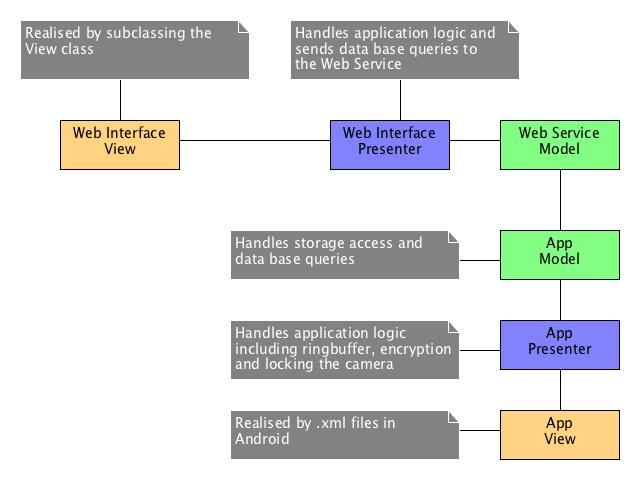
\includegraphics[scale=0.5]{./resources/Diagramme/overview_mvp.jpg}

Die Model-Rolle wird vom Web-Dienst erfüllt. Dieser bietet eine REST API, die sowohl vom Web Interface als auch von der App per HTTP-Anfragen angesprochen wird. Falls weitere Software entwickelt wird, mit der auf die Datenbank zugeriffen werden soll, soll diese ebenfalls auf die selbe API zugrifen können.\linebreak
Darüber hanus besitzt die App ein zusätzliches Model-Modul, das den Speicherzugriff regelt.\linebreak\par

Die Apllikationslogik wird durch die Presenter-Ebene umgesetzt. Hierbei besitzen App und Web Interface eigene Presenter-Module, die an die jeweilige Plattform angepasst sind. Der Presenter handhabt Eingaben durch Nutzer oder Sensoren und koordiniert die darauf folgenden Aktionen, wie das Ändern der Ansicht, Aktualisieren der Ansichten und den Zugriff auf die Model Ebene.\linebreak\par 

Die Rolle der View übernimmt schließlich die GUI. In Android wird diese durch entsprechende XML Dokumente implementiert, in Vaadin durch spezielle Java Klassen die von der Vaadin-Internen Klasse ``UI'' erben. Instanzierung, Manipulation und Navigation erfolgen schließlich durch die Presenter-Ebene, die Bindung erfolgt durch Beobachter und ist bereits durch das jewilige Framework festgelegt.



% PUT APP CONTENT HERE
\chapter{App} \label{chap:app}
\section{Architektur}

\begin{figure}[ht]
	\centering
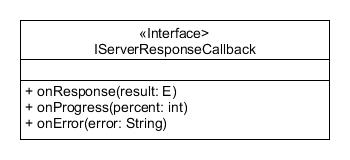
\includegraphics[width=1\textwidth]{./resources/Diagramme/App/UMLAndroidApp.jpg}
\caption{UML Diagram der Android App}
	\label{fig:modules_overview}
\end{figure}

\subsection{Entwurfsmuster}
\section{Datenhaltung}
Die App muss sich um die Verwaltung von Accountdaten, Einstellungen, Videos, Metadaten und symmetrischen Schlüsseln kümmern. 

\subsection{Nutzerdaten}
Für Accountdaten und  Einstllungen bieten sich die von Android bereitgestellten SharedPreferences an, die als Key-Value-Pairs aufgebaut werden. Das Schema ist in Schaubild \ref{fig:sharedpreferences_overview} veranschaulicht. Der Key entspricht den Daten die abgefragt werden sollen, also Einstellungen oder Account. Die gelesenen Werte bestehen jeweils aus einem String im JSON Format. Dadurch erreicht man eine Bündelung aller zusammengehörender Werte unter einem Key, unterstützt die Änderbarkeit und Ergänzbarkeit bestehender Daten und vereinfacht die Instanziierung von Account- und Einstellungen-Objekten durch einen Konstruktor, der einen JSON String entgegennimmt.\newline\par

\begin{figure}[ht]
	\centering
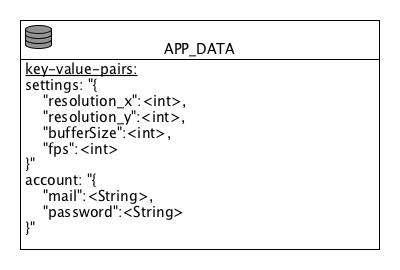
\includegraphics[width=0.5\textwidth]{./resources/Diagramme/App/SharedPreferences_overview.jpg}
\caption{Key-Value-Pairs der SharedPreferences}
	\label{fig:sharedpreferences_overview}
\end{figure}

\subsection{Dateien}
Für die Speicherung von Videos, Metadaten und symmetrischen Schlüsseln erweisen sich die SharedPreferences jedoch als ungeeignet. Hier gibt es zwei Lösungen: Entweder man speichert sie im internen oder im externen Speicher. Wir werden die erste Variante wählen, werden uns aber die Möglichkeit zum Exportieren der Daten in den externen Speicher frei halten. Der naive Ansatz merkt sich in den oben beschriebenen SharedPreferences die Namen aller gespeicherten Dateien und referenziert sie dadurch. Dabei ergibt sich aber folgendes Problem: Nachdem der Nutzer alle appinternen Daten gelöscht hat, hat man keine Chance mehr an extern gespeicherte Daten zu kommen. \newline\par
Wir verwenden einen generischeren Ansatz, der gänzlich auf die verwendung der SharedPreferences verzichtet: Es existieren drei Ordner: Ein Video-, ein Metadata- und ein Keyordner. Jedes Video erhält einen eindeutigen Namen, bestehend aus der exakten Aufnahmezeit. Jede mit diesem Video verwandte Datei, also dessen Metadaten und Schlüssel, besitzen den gleichen Dateinamen.\newline\par

Bezüglich der Metadaten muss auch beachtet werden, dass sie über die App ausgelesen werden können müssen, sie jedoch beim Speichervorgang des Videos direkt verschlüsselt werden um sie beim Hochladen des Videos verschlüsselt übertragen zu können. Aus diesem Grund werden die Metadaten in zwei Inhaltlich identische Dateien abgelegt. Eine der beiden wird veschlüsselt, die Andere nicht. An den Dateinamen der unverschlüsselten Datei wird zur identifikation schließlich ``\_readable'' angehängt\newline\par

Zusätzlich zu den erwähnten Ordnern existiert ein weiterer Ordner, der verwendet wird, um temporäre Videodateien abzulegen. Unter einer temporäre Videodatei ist hier ein unverschlüsseltes Video zu verstehen, welche nur zwischengespeichert wird. Android bietet hierzu die Möglichkeit, die temporäre Datei im appinternen Cache-Ordner abzulegen. Dies bietet außerdem den Vorteil, dass nur die App selbst Zugriff darauf hat.


\newpage
\section{Modulübersicht}
\subsection{Presenter}
\newpage
\section{Klassenübersicht}

\subsection{Presenter-Modul}
\subsubsection{CameraActivity} \label{app:klasse:CameraActivity}
\textbf{extends} \nameref{app:klasse:MainActivity} \newline
Die CameraActivity zeigt die CameraView an, instanzert eine CompatCameraHandler Instanz sowie eine IRecordCallback Instanz und manipuliert die graphische Nutzeroberfläche abhängig von den Methoden, die auf der IRecordCallback Instanz aufgerufen werden. Nach dem Start blendet die CameraActivity ein Symbol ein, welches die Bereitschaft der App signalisisert. Die CameraActivity stellt einen Observer des CompatCameraHandler dar.
\newline

\underline{Attribute}
\begin{itemize}
\itemsep0pt

\item \textbf{statusSymbol: ImageView} \hfill\\ 
\textbf{Sichtbarkeit} private\newline
ImageView die verwendet wird, um das Symbol einzublenden, welches die Bereitschaft bzw. die Aufnahme der App signalisiert.

\item \textbf{recordCallback: \nameref{app:klasse:IRecordCallback}} \hfill\\ 
\textbf{Sichtbarkeit} private\newline
Implementiert das IRecordCallback Interface. 
Der Aufruf der Mehtode \textit{onRecordStarted} benachrichtigt die CameraActivity Instanz über den Start der Videoaufnahme. Sie blendet das Symbol ein, welches die Aufnahme signalisiert. Das Symbol, welches zuvor die Bereitschaft der App signalisiert hat, wird ausgeblendet.
Der Aufruf der Methode \textit{onRecordStopped} benachrichtigt die CameraActivity Instanz über das Ende der Videoaufnahme. Sie blendet das Symbol ein, welches die Bereitschaft signalisiert. Das Symbol, welches zuvor die Aufnahme der App signalisiert hat, wird ausgeblendet.

\item \textbf{cameraHandler: \nameref{app:klasse:CompatCameraDataHandler}} \hfill\\ 
\textbf{Sichtbarkeit} private\newline
CameraHandler Instanz, die die Vorschaubilder der Kamera eigenständig verarbeitet und die Aufnahme auslößt. Diesem Feld wird eine TriggeringCompatCameraHandler Instanz zugewiesen.

\item \textbf{cameraView: \nameref{app:klasse:CameraView}} \hfill\\ 
\textbf{Sichtbarkeit} private\newline
CameraView Instanz, welche verwendet wird, um die Kameravorschau anzuzeigen.

\end{itemize}

\underline{Konstruktoren}\newline
\indent Keine, da der Lebenszyklus dieser Klasse von Android gesteuert wird.\newline

\underline{Methoden}
\begin{itemize}
\itemsep0pt

\item \textbf{Launch (callingActivity: Activity): void}\hfill\\
\textbf{Sichtbarkeit} public\newline
Startet ein neues Intent durch welches eine CameraActivity Instanz erzeugt und gestartet wird.

\item \textbf{getLayoutRes (): int}\hfill\\
\textbf{Sichtbarkeit} public\newline
Überschreibt die \textit{getLayoutRes} Methode der Superklasse.

\item \textbf{onCreate (savedInstanceState: Bundle): void}\hfill\\
\textbf{Sichtbarkeit} public\newline
Überschreibt die \textit{onCreate} Methode der Superklasse. Lädt die CameraView Instanz und erstellt die IRecorderCallback und CompatCameraHandler Instanzen.

\item \textbf{onResume (): void}\hfill\\
\textbf{Sichtbarkeit} public\newline
Überschreibt die \textit{onResume} Methode der Superklasse. Ruft die Methode \textit{setVisibility} der CameraView Instanz auf und übergibt den Parameter \textit{View.VISIBLE}.

\item \textbf{onPause (): void}\hfill\\
\textbf{Sichtbarkeit} public\newline
Überschreibt die \textit{onPause} Methode der Superklasse. Ruft die Methode \textit{setVisibility} der CameraView Instanz auf und übergibt den Parameter \textit{View.VISIBLE}.

\end{itemize}

\subsection{CameraLogic-Modul}

\subsection{MemoryAcess-Modul}

\subsection{ServerAcess-Modul}

\subsection{Utils-Modul}

% PUT WEB dienst CONTENT HERE
\chapter{Web-Dienst} \label{chap:service}
\section{Architektur}

\begin{figure}[ht]
	\centering
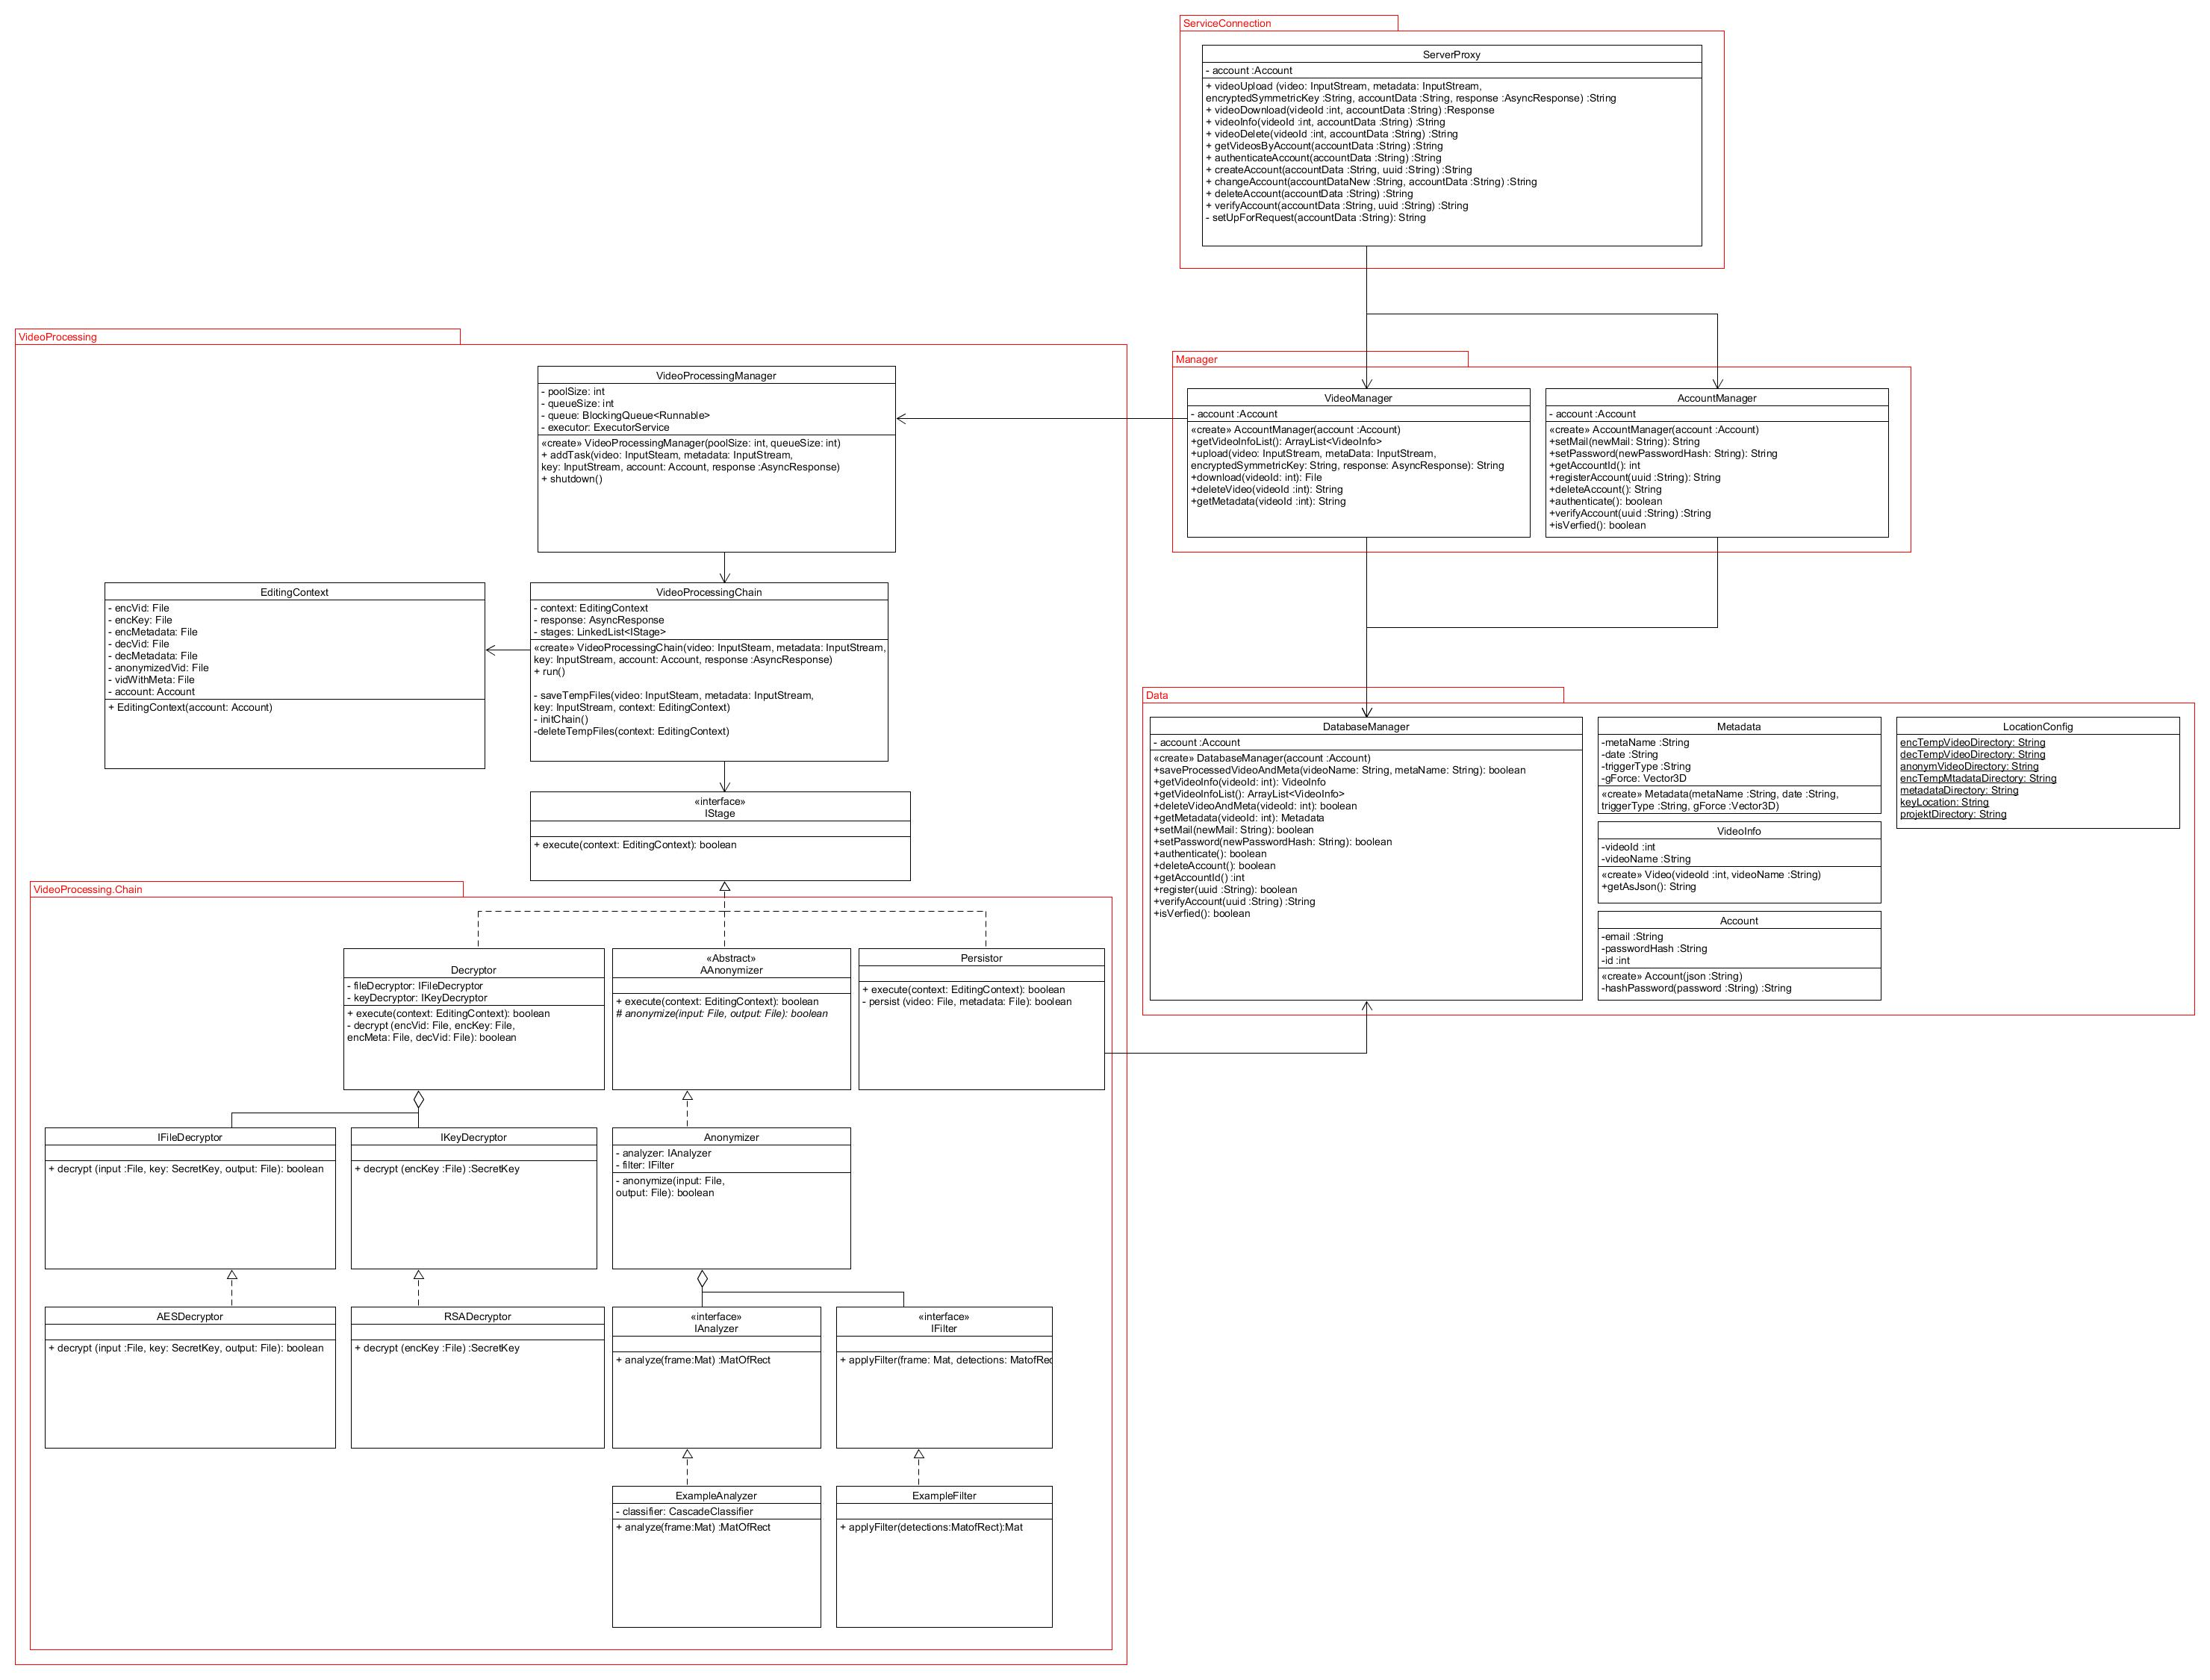
\includegraphics[width=1\textwidth]{./resources/Diagramme/Webservice/UMLSERVERPCC.jpg}
\caption{UML Diagramm des Web-Dienst}
	\label{service:fig:modules_overview}
\end{figure}

\subsection{Multithreading}
Um Anfragen vieler Nutzer unabhängig gleichzeitig zu bearbeiten, nimmt sich der Dienst für jede Anfrage einen einzelnen Thread. Unser verwendeter Webserver Jetty macht dies automatisch, indem er für jede Anfrage einen Thread aus einem internen ThreadPool nimmt, sofern vorhanden.\newline
Da die Bearbeitung der Videos jedoch sehr zeitaufwändig ist, lagern wie die Bearbeitung auf einen eigenen Worker ThreadPool um~\eqref{service:pattern:masterworker}, damit der Anfrage-Thread möglichst schnell seine Arbeit beenden kann und bereit für neue Anfragen ist. 

\subsection{Entwurfsmuster} \label{service:pattern}
Der Web-Service benutzt verschiedene Entwurfsmuster um vor allem zwei Ziele zu erreichen: 1. Eine schnelle und zeitlich unabhängige Bearbeitung von Anfragen und 2. Eine hohe Modularität und Austauschbarkeit.

\subsubsection{Proxy} \label{service:pattern:proxy}
Die Webanbindung des Services wird in dem \nameref{service:klasse:ServerProxy} gekapselt. Der Proxy bearbeitet bzw. verschickt lediglich die Http-Anfragen und leitet alle weitere Arbeit weiter. Dies sorgt für eine höhere Austauschbarkeit, da so die Webanbindung unabhängig von der eigentlichen Bearbeitung der Anfragen ausgetauscht werden kann und umgekehrt.

\subsubsection{Master-Worker} \label{service:pattern:masterworker}
Da die Bearbeitung der Videos auf dem Web-Dienst rechen- und damit zeitintensiv ist, nutzt er einen eigenen Worker-ThreadPool zur Bearbeitung der Videos. Dadurch muss der für die Serveranfrage verwendete Thread nur ein neues \nameref{service:klasse:VideoProcessingChain}-Objekt erzeugen und in die Warteschlange des \nameref{service:klasse:VideoProcessingManager} einreihen. Diese kann dann direkt zurückkehren um neue Anfragen entgegenzunehmen. Dies erlaubt dem Server schneller und mehr externe Anfragen anzunehmen, bevor dieser blockiert.\newline
Der VideoProcessingManager kann dann unabhängig von externen Anfragen auf seine eigenen Worker-Threads verteilen, um die Warteschlange abzuarbeiten.

\subsubsection{Pipeline} \label{service:pattern:pipeline}
Es gibt viele verschiedene Methoden Videos auf personenbezogene Daten zu analysieren. Dabei kann die Anzahl und Reihenfolge der durchlaufenen Arbeitsschritte stark variieren. Um den Web-Dienst in dieser Hinsicht möglichst flexibel zu gestalten, wird das Pipeline-Muster verwendet: \newline
Jeder Arbeitsschritt muss die einheitliche Schnittstelle \nameref{service:klasse:IStage} implementieren und somit eine Methode bereitstellen, die den Arbeitsschritt mithilfe des \nameref{service:klasse:EditingContext} ausführt.\newline
Die \nameref{service:klasse:VideoProcessingChain} besitzt eine Liste von Arbeitsschritten, die sie, sofern keine Fehler entstehen, der Reihe nach ausführt. In diese Liste können jeder Zeit Arbeitsschritte eingefügt bzw. entfernt werden, die Reihenfolge der Arbeitsschritte verändert, oder der komplette Ablauf ausgetauscht werden. Theoretisch sind sogar Änderungen zur Laufzeit möglich.\newline
Durch die Kapselung der Arbeitsschritte in einzelne Klassen ist es zudem möglich Arbeitsschritte in verschiedenen Ausführungsreihenfolgen wiederzuverwenden ohne, dass erneuter Initialisierungsaufwand entsteht.

\subsubsection{Strategie} \label{service:pattern:strategie}
Da es für das, von uns bereitgestellte Bearbeitungschema für Videos, viele verschiedene Algorithmen für die einzelnen Schritte gibt, wird das Strategie-Muster verwendet:\newline
Für die Schritte, die man eventuell austauschen möchte (z.B den Filter mit dem Bildbereiche unkenntlich gemacht werden) existiert eine Schnittstelle (z.B \nameref{service:klasse:IFilter}). Dann können nach belieben konkrete Implementierungen (hier z.B. \nameref{service:klasse:ExampleFilter}) ausgetauscht werden, indem man bei der aufrufenden Klasse (hier: \nameref{service:klasse:AAnonymizer}). Theoretisch ist dies sogar zur Laufzeit möglich.
\newpage
\section{Datenhaltung}
Die Daten des Web-Dienstes werden in einer Datenbank und in Ordnern organisiert. 
Nutzerdaten und Videodaten werden in Tabellen gespeichert. Als Syntax wird PostgreSQL verwendet. 

\begin{figure}[ht]
	\centering
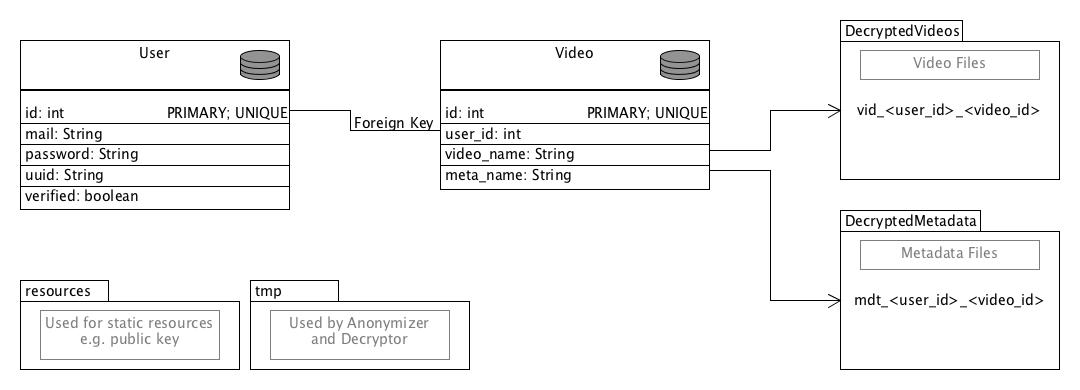
\includegraphics[width=1\textwidth]{./resources/Diagramme/Webservice/database_scheme.jpg}
\caption{Datenbankschema}
	\label{fig:overview_mvp}
\end{figure}

\subsection{Datenbank}

Die User-Tabelle für die Nutzerdaten speichert eine einzigartige Nutzer-Id, die Mail-Adresse, das Passwort und ob der Nutzer bereits seinen Account verifiziert hat.\newline
Die Video-Tabelle für Videodaten speichert eine einzigartige  Video-Id, die Nutzer-Id des Nutzers, der das Video hochgeladen hat sowie den Videodateiname und den Metadatendateiname. die Nutzer-Id agiert hier als Fremdschlüssel, die Dateinamen werden zum referenzieren der Dateien aus den Ordnern verwendet.\newline
Video und Metadaten werden in jeweils einem eigenen Ordner organisiert. Dabei teilen sich Videodateien aller Nutzer einen Ordner und Metadatendateien aller Nutzer einen Ordner. Der Dateiname wird stets aus einem statischen Anfang und der Kombination aus Nutzer-Id und Video-Id zusammengesetzt und ist daher einzigartig.

\subsection{Temporäre Dateien}
Die Verwaltung der temporären Dateien für die Bearbeitung der Videos übernimmt das \nameref{service:modul:VideoProcessing} Modul. Dies ist notwendig, da die entstehenden und benötigten Daten ausschließlich abhängig von den Arbeitsschritten der \nameref{service:klasse:VideoProcessingChain} ist und daher nicht von anderen Modulen des Web-Dienstes beeinflusst werden soll. Der Web-Dienst stellt dafür den \textit{tmp} Ordner bereit. Es existieren keine Schnittstellen um von außen direkt auf Inhalte dieses Ordners zuzugreifen.\newline
Der \nameref{service:klasse:EditingContext} erzeugt dann alle für die Bearbeitung notwendigen Dateipfade in der Form:\newline
\textit{benutzerid\_videoname\_attribut.endung}

\subsection{Verwendete Resourcen}
Für die Bearbeitung der Videos verwendete Ressourcen (z.B. der private Key des \nameref{service:klasse:RSADecryptor} oder der CascadeClassifier des \nameref{service:klasse:ExampleAnalyzer}) werden im "'resources"' Ordner abgelegt.
\newpage
\section{Modulübersicht} \label{service:modul}

\begin{figure}[ht]
	\centering
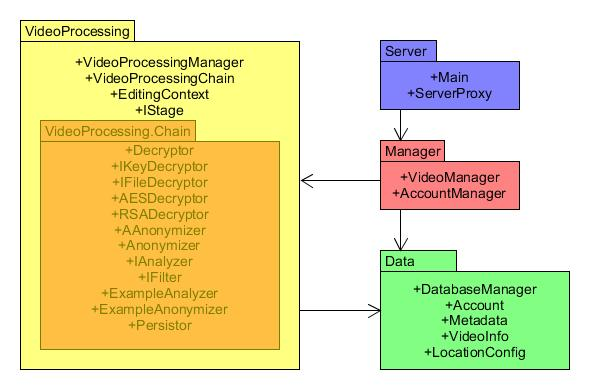
\includegraphics[width=1\textwidth]{./resources/Diagramme/Webservice/modules_overview.jpg}
\caption{Modulübersicht}
	\label{fig:modules_overview}
\end{figure}
\subsection{Server} \label{service:modul:Server}
Das Server Modul ist für das starten und verwalten des Servers zuständig. Außerdem empfängt es die Webanfragen von \nameref{chap:app} und \nameref{chap:interface}, entpackt sie und leitet sie an die bearbeitenden Klassen weiter.
\subsection{Data} \label{service:modul:Data}
Das Data-Modul ist für die Verwaltung der Daten auf der Datenbank da und bietet eine Reihe von Hilfsklassen an, die das Behandeln von zusammengehörenden Daten vereinfacht.
\subsection{Manager} \label{service:modul:Manager}
Das Manager-Paket beinhaltet die Presenter-Klassen des Web-Dienstes. Diese dienen dazu die Bearbeitung von Anfragen zu initiieren. So werden Accounts angelegt oder überprüft, hochgeladene Videos zur Bearbeitung weitergegeben, oder Informationen aus der Datenbank abgefragt.

\subsection{VideoProcessing} \label{service:modul:VideoProcessing}
Das VideoProcessing-Modul ist ein elementares Modul der Privacy-Crash-Cam. Es ist für die Anonymisierung der, von der \nameref{chap:app} hochgeladenen Videos zuständig.\newline
Das Modul ist in ein Haupt- und ein Unterpaket gegliedert. Das Hauptpaket übernimmt die Verwaltung der Anfragen und die Verteilung der Rechenarbeit auf die vorhandenen Ressourcen. Das Unterpaket \nameref{service:modul:VideoProcessingChain} beinhaltet alle Klassen, die die Bearbeitung des Videos umsetzen.
\subsection{VideoProcessing.Chain} \label{service:modul:VideoProcessingChain}
Das Paket VideoProcessing.Chain beinhaltet alle Klassen, die von der \nameref{service:klasse:VideoProcessingChain} verwendet werden um ein hochgeladenes Video zu bearbeiten.
\newpage
\section{Klassenübersicht}

\subsection{Server}
\subsubsection{Main} \label{service:klasse:Main}
Die Klasse Main ist der Haupteinstiegspunkt des Web-Dienstes. Sie sorgt dafür bei Serverstart alles korrekt zu starten und ist dafür zuständig den Server zu stoppen und neuzustarten.\newline

\underline{Attribute}
\begin{itemize}
\itemsep0pt
\item \textbf{server: Server} \hfill\\ 
\textbf{Sichtbarkeit} private \newline
\textbf{static}

Server des Web-Dienstes.

\item \textbf{LOGGER: Logger} \hfill\\ 
\textbf{Sichtbarkeit} public \newline
\textbf{static}

Globaler Logger des Web-Dienstes.

\item \textbf{PORT: Server} \hfill\\ 
\textbf{Sichtbarkeit} private \newline
\textbf{static}

Port des Servers.
\end{itemize}

\underline{Methoden}
\begin{itemize}
\itemsep0pt
\item \textbf{main (args: String[ ]): void}\hfill\\
\textbf{Sichtbarkeit} public \newline
\textbf{statisch}

Haupteinstiegspunkt des Web-Dienstes. Startet den Logger, erstellt alle Ordner falls nötig und löscht die temporären Dateien.

\item \textbf{stopServer (): void}\hfill\\
\textbf{Sichtbarkeit} public \newline
\textbf{statisch}

Stoppt den Server.


\item \textbf{restartServer (): void}\hfill\\
\textbf{Sichtbarkeit} public \newline
\textbf{statisch}

Stoppt den Server setzt ihn neu auf und startet ihn wieder.

\item \textbf{setupLogger (): void}\hfill\\
\textbf{Sichtbarkeit} private \newline
\textbf{statisch}

Konfiguriert den globalen Logger und startet ihn.


\item \textbf{setupDirectories (): void}\hfill\\
\textbf{Sichtbarkeit} private \newline
\textbf{statisch}

Erstellt alle benötigten Ordner, falls diese noch nicht vorhanden sind und löscht alle temporären Dateien.


\item \textbf{startServer (): void}\hfill\\
\textbf{Sichtbarkeit} private \newline
\textbf{statisch}

Konfiguriert und startet den Server.

\end{itemize}
\newpage

\subsubsection{ServerProxy} \label{service:klasse:ServerProxy}
Der ServerProxy ist die Schnittstelle zwischen \nameref{chap:service} und \nameref{chap:interface}/\nameref{chap:app}. Die Anfragen an den ServerProxy werden mittels der REST-API übermittelt. Die Anfragen werden in Teilanfragen aufgespalten und mithilfe des \nameref{service:modul:Manager}-Moduls weiter bearbeitet. \newline
Siehe auch: \nameref{fig:ServiceAuth}, \nameref{fig:ServiceUpload}, \nameref{fig:ServiceDownl}, \nameref{fig:ServiceDel}

\underline{Attribute}
\begin{itemize}
\itemsep0pt
\item \textbf{account: \nameref{service:klasse:Account}} \hfill\\ 
\textbf{Sichtbarkeit} private

Instanz des Accounts, der die Anfrage geschickt hat. Wird in der Methode setUpForRequest() initialisiert.
\end{itemize}

\underline{Konstruktoren}
\begin{itemize}
\itemsep0pt
\item \textbf{ServerProxy()} \hfill\\
Standardkonstruktor
\end{itemize}

\underline{Methoden}
\begin{itemize}
\itemsep0pt
\item \textbf{videoUpload (video: InputStream, metadata: InputStrem, encryptedSymmetricKey: String, accountData: String, response: AsyncResponse): String}\hfill\\
\textbf{Sichtbarkeit} public

Bearbeitet eine VideoUpload Anfrage der App. Übergibt die videobezogenen Parameter (video, metadata und encryptedSymmetricKey) und die AsyncResponse an die upload()-Methode im \nameref{service:klasse:VideoManager}. Die Rückgabe als JSON-String gibt an, ob die Dateien vollständig angekommen sind. 

\item \textbf{videoDownload(videoId: int, accountData: String): Response}\hfill\\
\textbf{Sichtbarkeit} public

Leitet einen Download-Anfrage ein. Gibt die VideoId an die download()-Methode des VideoManagers weiter. Mithilfe der Id wird dann das gesuchte Video gefunden. Die Response-Rückgabe ermöglicht den bekannten Download-Dialog auf dem Interface.

\item \textbf{videoInfo(videoId: int, accountData: String): String}\hfill\\
\textbf{Sichtbarkeit} public

Bearbeitet eine Anfrage zur Informationsausgabe eines Videos des Web-Interfaces. Dabei werden die Metadaten des zugehörigen Videos über den VideoManager mithilfe der VideoId gefunden. Die String Rückgabe beinhaltet die relevanten Video Informationen.

\item \textbf{videoDelete(videoId: int, accountData: String): String}\hfill\\
\textbf{Sichtbarkeit} public

Bearbeitet eine Anfrage zum Löschen eines Videos des Web-Interfaces. Diese wird über die deleteVideo()-Methode des VideoManagers weiter bearbeitet. Die String Rückgabe gibt Meldung über das Ergebnis der Anfrage.

\item \textbf{getVideosByAccount(accountData: String): String}\hfill\\
\textbf{Sichtbarkeit} public  

Bearbeitet eine Anfrage zur Videolistenrückgabe des Web-Interface für einen bestimmten Nutzer. Dabei wird im VideoManager die getVideoListMethode aufgerufen. Diese bearbeitet die Anfrage und gibt einen JSON-String mit den Videoinformationen zurück. Dieser JSON-String wird aus dem ArrayList<VideoInfo> erstellt. Diese werden dann auch an das Web-Interface zurückgegeben. 

\item \textbf{authenticateAccount(accountData: String): String}\hfill\\
\textbf{Sichtbarkeit} public

Bearbeitet eine Anfrage zur Authentifizierungs des Web-Interfaces oder App. Dabei wird auf die Rückgabe von setUpForRequest() gewartet und der String dann an die anfragende Instanz weitergeleitet.

\item \textbf{createAccount(accountData: String uuid :String): String}\hfill\\
\textbf{Sichtbarkeit} public

Bearbeitet eine Anfrage zur Accounterstellung des Web-Interfaces. Die Die Übergabe ``uuid'' stellt eine Eindeutige id des Accounts dar, die zur Accountverifizierung dient. Dabei wird im \nameref{service:klasse:AccountManager} die Methode registerAccount(uuid :String) aufgerufen. Die Rückgabe gibt Meldung über das Ergebnis der Anfrage an das Web-Interface.

\item \textbf{changeAccount(accountDataNew: String, accountData: String): String}\hfill\\
\textbf{Sichtbarkeit} public

Bearbeitet eine Anfrage zur Passwort/Mailänderung des Web-Interfaces. Dabei werden im AccountManager die Methoden setMail() und setPassword()  aufgerufen. Die Rückgabe gibt Meldung über das Ergebnis der Anfrage an das Web-Interface.

\item \textbf{deleteAccount(accountData: String): String}\hfill\\
\textbf{Sichtbarkeit} public

Bearbeitet eine Anfrage zur Löschung eines Accounts des Web-Interfaces. Es wird im AccountManager die Methode deleteAccount(vM :VideoManager) aufgerufen. Die Rückgabe gibt Meldung über das Ergebnis der Anfrage an das Web-Interface.

\item \textbf{verifyAccount(accountData :String, uuid: String): String}\hfill\\
\textbf{Sichtbarkeit} public

Bearbeitet eine Anfrage zur Verifizierung der E-Mail eines Accounts. Die Übergabe ``uuid'' stellt eine eindeutige Id des Accounts dar. Die Methode gibt einen JSON-String mit dem Ergebnis zurück.

\item \textbf{setUpForRequest(accountData: String)}\hfill\\
\textbf{Sichtbarkeit} private

Bei jeder Anfrage wird zu Beginn die private Methode setUpForRequest() aufgerufen, um die Klassen des Manager-Moduls zu initialisieren und die Authentifizierung des Accounts zu gewährleisten. Die Rückgabe gibt Meldung über das Ergebnis der Authentifizierung des Accounts. Die Authentifizierung ruft im AccountManager die Methoden getAccountId(), authenticate() und isVerified() auf.
\end{itemize}
\newpage

\subsection{Data}
\subsubsection{DatabaseManager} \label{service:klasse:DatabaseManager}
Die Klasse DatabaseManager bietet eine Schnittstelle für alle Datenbankanfragen, die vom \nameref{service:klasse:AccountManager} und \nameref{service:klasse:VideoManager} benötigt wird. \hfill\\

\underline{Attribute}
\begin{itemize}
\itemsep0pt
\item \textbf{account: Account} \hfill\\ 
\textbf{Sichtbarkeit} private

Benutzeraccount des aktiven Nutzers.
\end{itemize}

\underline{Konstruktoren}
\begin{itemize}
\itemsep0pt
\item \textbf{DatabaseManager(account: \nameref{service:klasse:Account})} \hfill\\
Setzt den aktiven Nutzer.
\end{itemize}

\underline{Methoden}
\begin{itemize}
\itemsep0pt
\item \textbf{saveProcessedVideoAndMeta(videoName: String, metaName: String): boolean}\hfill\\
\textbf{Sichtbarkeit} public

Bekommt den Videofile-Namen, sowie die Metadaten als übergeben und schreibt einen Datenbank-Eintrag in die Video-Tabelle der Datenbank. Die ``id'' wird generiert, die ``user\_id'' ist das Attribut ``id'' des Account-Objektes, der ``video\_name'' ist der Übergabeparameter ``videoName'' und ``meta\_name'' ist der Übergabeparameter ``metaName''.

\item \textbf{getVideoInfo(videoId: int): \nameref{service:klasse:VideoInfo}}\hfill\\
\textbf{Sichtbarkeit} public

Bekommt die videoId übergeben und gibt Videoinformationen als \nameref{service:klasse:VideoInfo}-Objekt zurück. Die Daten werden mithilfe der videoId und den Accountdaten des Nutzers aus der Datenbank geladen.

\item \textbf{getVideoInfoList(): ArrayList<VideoInfo>}\hfill\\
\textbf{Sichtbarkeit} public

Gibt alle Videos eines Benutzers in Form einer Liste von ``VideoInfo''-Objekten zurück. Diese wird durch eine Datenbankabfrage mithilfe der Accountdaten ermittelt.

\item \textbf{deleteVideoAndMeta(videoId: int): boolean}\hfill\\
\textbf{Sichtbarkeit} public

Löscht ein Video eines Benutzers. Das Löschen geschieht durch eine Datenbankabfrage mithilfe der videoId und den Accountdaten des aktiven Benutzers. Die Methode gibt zurück, ob das Löschen erfolgreich war.

\item \textbf{getMetadata(videoId: int): \nameref{service:klasse:Metadata}}\hfill\\
\textbf{Sichtbarkeit} public

Ermittelt die Metadaten eines Videos durch eine Datenbankabfrage. Dafür wird die videoId und die Benutzerdaten genutzt.

\item \textbf{setMail(newMail: String): boolean}\hfill\\
\textbf{Sichtbarkeit} public

Die Methode ändert die E-Mail-Adresse des Benutzers. Die E-Mail-Adresse wird als ``newMail'' übergeben und mithilfe des Accounts kann auf das Element in der Datenbank zugegriffen werden. Mit dem entsprechenden Datenbankbefehl wird die neue E-Mail gesetzt. Es wird zurückgegeben, ob das aktualisieren erfolgreich war, oder nicht.

\item \textbf{setPassword(newPassword: String): boolean}\hfill\\
\textbf{Sichtbarkeit} public

Die Methode ändert das Passwort des Benutzers. Der neue Passwort-Hash wird als Parameter ``newPasswordHash'' übergeben und mithilfe des Accounts kann durch ein Datenbankbefehl der neue Passwort-Hash gesetzt werden. Ein ``boolean'' wird zurückgegeben, je nachdem, ob die Operation erfolgreich war oder nicht.

\item \textbf{authenticate(): boolean}\hfill\\
\textbf{Sichtbarkeit} public

Die Methode authentifiziert den Benutzer. Durch das den Account stehen alle benötigten Informationen zur Verfügung. Durch eine Datenbankabfrage wird überprüft, ob E-Mail und Passwort-Hash übereinstimmen. Es wird zurückgegeben, ob das aktualisieren erfolgreich war, oder nicht.

\item \textbf{deleteAccount(): boolean}\hfill\\
\textbf{Sichtbarkeit} public

Die Methode löscht einen Account. Durch den Account stehen alle Informationen zur Verfügung. Zunächst werden alle Videos und Metadaten des Nutzers gelöscht. Danach werden die Video-Datenbankeinträge in der Tabelle ``Video'' und dann der Account in der Tabelle ``User'' gelöscht.

\item \textbf{getAccountId() :int}\hfill\\
\textbf{Sichtbarkeit} public

Die Methode gibt die ``id'' des Accounts zurück. Diese ermittelt sie durch eine Datenbankabfrage mit der Adresse des Accounts. Falls der Account nicht existiert, wird ``-1'' zurückgegeben.

\item \textbf{register(uuid :String) :boolean}\hfill\\
\textbf{Sichtbarkeit} public

Die Methode legt einen neuen Benutzer an. Die Die Übergabe ``uuid'' ist ein eindeutiger Wert, der zur Accountverifizierung dient. Die zur Erstellung des Account benötigten Informationen liegen in dem Attribut account vor. Daraus werden E-Mail und Passwort genommen und mit einer Datenbankabfrage wird in der Tabelle ``User'' ein neuer Eintrag hinzugefügt. 

\item \textbf{verifyAccount(accountData :String, uuid: String): String}\hfill\\
\textbf{Sichtbarkeit} public

Bearbeitet eine Anfrage zur Verifizierung der E-Mail eines Accounts. Die Übergabe ``uuid'' stellt eine eindeutige Id des Accounts dar. Die Methode gibt einen JSON-String mit dem Ergebnis zurück.

\item \textbf{isVerfied(): boolean}\hfill\\
\textbf{Sichtbarkeit} public

Die Methode überprüft, ob ein Nutzer verifiziert ist.

\end{itemize}
\newpage

\subsubsection{Account} \label{service:klasse:Account}
Die Klasse Account repräsentiert den Account eines Benutzers. \newline

\underline{Attribute}
\begin{itemize}
\itemsep0pt
\item \textbf{email: String} \hfill\\ 
\textbf{Sichtbarkeit} private 

E-Mail-Adresse des Accounts.

\item \textbf{passwordHash: String} \hfill\\ 
\textbf{Sichtbarkeit} private 

PasswordHash des Accounts.

\item \textbf{id: int} \hfill\\ 
\textbf{Sichtbarkeit} private  

Die ``id'' ist identisch der ``id'' in der Tabelle User der Datenbank.

\end{itemize}

\underline{Konstruktoren}
\begin{itemize}
\itemsep0pt
\item \textbf{Account(json: String)} \hfill\\
\textbf{Sichtbarkeit} public

Der Konstruktor nimmt ein JSON-Objekt entgegen, wertet die Informationen aus und setzt die Attribute. Die Information ``password'' wird mit der Methode ``hashPassword(password: String)'' gehasht und dann gesetzt.

\end{itemize}

\underline{Methoden}
\begin{itemize}
\itemsep0pt
\item \textbf{hashPassword(password: String): String}\hfill\\
\textbf{Sichtbarkeit} private

Die Methode nimmt das im Klartext gegebene Passwort und hasht dieses.

\end{itemize}
\newpage

\subsubsection{Metadata} \label{service:klasse:Metadata}
Die Klasse Metadata beinhaltet alle wichigen Informationen zu den Metadaten eines Videos. \newline

\underline{Attribute}
\begin{itemize}
\itemsep0pt
\item \textbf{date: String} \hfill\\ 
\textbf{Sichtbarkeit} private 

Datum, an dem das Video aufgenommen wurde.

\item \textbf{triggerType: String} \hfill\\ 
\textbf{Sichtbarkeit} private 

Art, wie das Video ausgelöst wurde (G-Sensor, manuelle Auslösung). 

\item \textbf{gForce: Vector3D} \hfill\\ 
\textbf{Sichtbarkeit} private 

Messwerte des G-Sensors zum Auslösezeitpunkt.

\end{itemize}

\underline{Konstruktoren}
\begin{itemize}
\itemsep0pt
\item \textbf{Metadata(metaName :String, date :String, triggerType :String, gForce :Vector3D)} \hfill\\
\textbf{Sichtbarkeit} public 

Weist die Parameter den Attributen zu

\end{itemize}

\underline{Methoden}
\begin{itemize}
\itemsep0pt
\item \textbf{getAsJson(): String}\hfill\\
\textbf{Sichtbarkeit} public 

Die Methode gibt ein JSON-String zurück, welcher aus den Informationen aller Klassenattributen zusammengesetzt wird.

\end{itemize}
\newpage

\subsubsection{VideoInfo} \label{service:klasse:VideoInfo}
Die Klasse VideoInfo beinhaltet die benötigten Informationen zum Video.\newline

\underline{Attribute}
\begin{itemize}
\itemsep0pt
\item \textbf{videoId: int} \hfill\\ 
\textbf{Sichtbarkeit} private \hfill\\  

Die ``videoId'' ist die ``videoId'' des zugehörigen Datenbankeintrags.

\item \textbf{videoName: String} \hfill\\ 
\textbf{Sichtbarkeit} private \hfill\\ 

Der ``videoName'' ist der Name des Videos im zugehörigen Datenbankeintrag.

\end{itemize}

\underline{Konstruktoren}
\begin{itemize}
\itemsep0pt
\item \textbf{Video(videoId: int, videoName: String)} \hfill\\

Weist die Parameterübergabe den zugehörigen Klassenattributen zu.

\end{itemize}

\underline{Methoden}
\begin{itemize}
\itemsep0pt
\item \textbf{getAsJson(): String}\hfill\\
\textbf{Sichtbarkeit} public

Die Methode gibt ein JSON-String zurück, der aus den Informationen aller Klassenattributen zusammengesetzt wird.

\end{itemize}
\newpage

\subsubsection{LocationConfig} \label{service:klasse:LocationConfig}
Die Klasse LocationConfig beinhaltet alle Pfade als statischen Strings, die für das Projekt benötigt werden.

\underline{Attribute}
\begin{itemize}
\itemsep0pt
\item \textbf{encTempVideoDirectory: String} \hfill\\ 
\textbf{Sichtbarkeit} public

Das Klassenattribut ist ein statisches Attribut und beinhaltet den Pfad zu allen verschlüsselten Videos.

\item \textbf{decTempVideoDirectory: String} \hfill\\ 
\textbf{Sichtbarkeit} public
 
Das Klassenattribut ist ein statisches Attribut und beinhaltet den Pfad zu allen entschlüsselten Videos.

\item \textbf{anonymVideoDirectory: String} \hfill\\ 
\textbf{Sichtbarkeit} public

Das Klassenattribut ist ein statisches Attribut und beinhaltet den Pfad zu allen anonymisierten Videos.

\item \textbf{encTempMetadataDirectory} \hfill\\ 
\textbf{Sichtbarkeit} public

Das Klassenattribut ist ein statisches Attribut und beinhaltet den Pfad zu allen verschlüsselten temporär abgelegten Metadaten.

\item \textbf{metadataDirectory: String} \hfill\\ 
\textbf{Sichtbarkeit} public

Das Klassenattribut ist ein statisches Attribut und beinhaltet den Pfad zu allen entschlüsselten Metadaten.

\item \textbf{keyDirectory: String} \hfill\\ 
\textbf{Sichtbarkeit} public

Das Klassenattribut ist ein statisches Attribut und beinhaltet den Pfad zu der Directory der Keys.
\end{itemize}
\newpage

\subsection{Manager}
\subsubsection{AccountManager} \label{service:klasse:AccountManager}
Verbindet zwischen dem \nameref{service:modul:Data}-Modul und dem \nameref{service:modul:Server}-Modul. Er bearbeitet die Anfragen des \nameref{service:klasse:ServerProxy}s und gibt die gefragten Ergebnisse zurück. \newline

\underline{Attribute}
\begin{itemize}
\itemsep0pt
\item \textbf{account: \nameref{service:klasse:Account}} \hfill\\ 
\textbf{Sichtbarkeit} public

Account-Instanz, welche zur Bearbeitung der verschiedenen Anfragen benötigt wird.
\end{itemize}

\underline{Konstruktoren}
\begin{itemize}
\itemsep0pt
\item \textbf{AccountManager(account: Account)} \hfill\\
\textbf{Sichtbarkeit} public

Erstellt eine Instanz eines AccountManagers mit dem dazugehörigen Account. Dieser wird vom ServerProxy über die Parameter übergeben und dann gesetzt.
\end{itemize}

\underline{Methoden}
\begin{itemize}
\itemsep0pt
\item \textbf{setMail(newMail: String): String}\hfill\\
\textbf{Sichtbarkeit} public

Bearbeitet eine Anfrage vom ServerProxy zur Ersetzung einer Mail eines Accounts. Die übergebene Mail wird dann im \nameref{service:klasse:DatabaseManager} mit der Methode setMail() gesetzt.

\item \textbf{setPassword(newPasswordHash: String): String}\hfill\\
\textbf{Sichtbarkeit} public

Bearbeitet eine Anfrage vom ServerProxy zur Ersetzung eines Passwort eines Accounts. Das übergebene Passwort wird dann im DatabaseManager mit der Methode setPassword() gesetzt.

\item \textbf{getAccountId(): int}\hfill\\
\textbf{Sichtbarkeit} public

Bearbeitet eine Anfrage vom ServerProxy zur Bestimmung der AccountId zu einer Mail-Adresse. Die Anfrage wird zum DatabaseManager weitergeleitet und somit die Methode getAccountId() aufgerufen. Von dort aus wird sie bis zum ServerProxy zurückgegeben.  

\item \textbf{registerAccount(uuid :String): String}\hfill\\
\textbf{Sichtbarkeit} public

Bearbeitet eine Anfrage vom ServerProxy zur Accountregistrierung. Die Die Übergabe ``uuid'' stellt eine eindeutige Id des Accounts dar, die zur Accountverifizierung dient. Dabei wird beim DatabaseManager die Methode register() aufgerufen und die Accountdaten im zugehörigen Accountattribut gesetzt. 

\item \textbf{deleteAccount(vm :VideoManager): String}\hfill\\
\textbf{Sichtbarkeit} public

Bearbeitet die Löschung eines Accounts. Zunächst werden alle Videos des Accounts ermittelt und es wird mit dem Übergabeparameter ``vM'' auf den \nameref{service:klasse:VideoManager} zugegriffen, der alle Videos und Metadaten löscht. Nun wird im DatabaseManager ``deleteAccount()'' aufgerufen und der Account wird in der Datenbank gelöscht.

\item \textbf{authenticate(): boolean}\hfill\\
\textbf{Sichtbarkeit} public

Bearbeitet eine Anfrage vom ServerProxy zur Authentifizierung des Accounts. Die Methode authenticate() vom DatabaseManager wird hierbei aufgerufen.
 
\item \textbf{verifyAccount(accountData :String, uuid: String) :String}\hfill\\
\textbf{Sichtbarkeit} public

Bearbeitet eine Anfrage zur Verifizierung der E-Mail eines Accounts. Die Übergabe ``uuid'' stellt eine eindeutige Id des Accounts dar. Die Methode gibt einen JSON-String mit dem Ergebnis zurück. 
 
\item \textbf{isVerfied(): boolean}\hfill\\
\textbf{Sichtbarkeit} public

Bearbeitet eine Anfrage vom ServerProxy zum Verifizierungsstatus eines Accounts. Die Anfrage wird zum DatabaseManager weitergeleitet und die Methode isVerified() aufgerufen. Von dort wird der boolean bis zum ServerProxy zurückgegeben.
\end{itemize}
\newpage

\subsubsection{VideoManager} \label{service:klasse:VideoManager}
Der VideoManager verbindet zwischen dem \nameref{service:modul:Server}-Modul und dem \nameref{service:modul:Data}- bzw. \nameref{service:modul:VideoProcessing}-Modul. Er bearbeitet die Anfragen des \nameref{service:klasse:ServerProxy}s und gibt die gefragten Ergebnisse zurück.\newline
Siehe auch: \nameref{fig:ServiceDownl}, \nameref{fig:ServiceDel}, \nameref{fig:ServiceUpload} \newline

\underline{Attribute}
\begin{itemize}
\itemsep0pt
\item \textbf{account: \nameref{service:klasse:Account}} \hfill\\ 
\textbf{Sichtbarkeit} private 

Account-Instanz, welche zur Bearbeitung der verschiedenen Anfragen benötigt wird.

\end{itemize}

\underline{Konstruktoren}
\begin{itemize}
\itemsep0pt
\item \textbf{VideoManager(account :Account)} \hfill\\
\textbf{Sichtbarkeit} public

Erstellt eine Instanz eines \nameref{service:klasse:VideoManager}s mit dem dazugehörigen Account. Dieser wird vom ServerProxy über die Parameter übergeben und dann gesetzt.
\end{itemize}

\underline{Methoden}
\begin{itemize}
\itemsep0pt
\item \textbf{getVideoInfoList(): ArrayList<VideoInfo>}\hfill\\
\textbf{Sichtbarkeit} public

Bearbeitete eine Anfrage vom ServerProxy zur Videolistenrückgabe eines Accounts. Dabei wird im DatabaseManager die Methode getVideoInfoList() aufgerufen. Die ArrayList Der \nameref{service:klasse:VideoInfo}-Objekte wird dann an den ServerProxy zurückgegeben.    

\item \textbf{upload(video: InputStream, metaData: InputStream,
encryptedSymmetricKey: String, response: AsyncResponse): String}\hfill\\
\textbf{Sichtbarkeit} public

Bearbeitet eine Anfrage vom ServerProxy zum Hochladen mehrerer Dateien. Da der Upload komplett vom VideoProcessing-Modul übernommen wird, werden hier alle übergebenen Parameter und der Account beim Aufruf der Methode addTask() vom VideoProcessingManager übergeben.

\item \textbf{download(videoId: int): File}\hfill\\
\textbf{Sichtbarkeit} public

Bearbeitet eine Anfrage vom ServerProxy zum Herunterladen eines Videos. Dabei wird vom DatabaseManager die Methode getVideoInfo() aufgerufen, um mittels der VideoId den Videonamen über das VideoInfo Objekt zu bekommen. Somit kann dann das gewünschte File gefunden und zurückgegeben werden.

\item \textbf{deleteVideo(videoId :int): String}\hfill\\
\textbf{Sichtbarkeit} public

Bearbeitet eine Anfrage vom SererProxy zum Löschen eines Videos. Zunächst wird die Methode getVideoInfo() und getMetadata() des DatabaseManagers aufgerufen. Somit bekommen wir über das VideoInfo-Objekt und \nameref{service:klasse:Metadata}-Objekt den Videonamen und Metadatanamen und können diese Files löschen. Daraufhin wird die Methode deleteVideoAndMeta() des DatabaseMangers aufgerufen, welche die beiden Einträge aus der Datenbank löscht.

\item \textbf{getMetadata(videoId :int): String}\hfill\\
\textbf{Sichtbarkeit} public

Bearbeitet die Anfrage vom ServerProxy zum Ausgeben der Metadata eines Videos. Es wird im DatabaseManager die Methode getMetadata() aufgerufen, die ein Metadata-Objekt zurückgibt. Die relevanten Attribute werden in ein JSON-String umgewandelt und dann an den ServerProxy zurückgeben.
\end{itemize}
\newpage

\subsection{VideoProcessing}
\subsubsection{VideoProcessingManager} \label{service:klasse:VideoProcessingManager}
Der VideoProcessingManager ist dafür zuständig, die Bearbeitung der hochgeladenen Videos zu koordinieren und auf seine Worker-Threads zu verteilen. Nachdem er vom \nameref{service:klasse:VideoManager} eine Anfrage erhalten hat wird eine \nameref{service:klasse:VideoProcessingChain} erzeugt und in die Warteschlange des Managers eingereiht, aus der die Worker-Threads kontinuierlich Anfragen abarbeiten. Das Ganze passiert asynchron zu der ursprünglichen Anfrage, damit das aufwändige Bearbeiten der Videos nicht die Serveranfragen aufhält. Dafür werden die von der Java API bereitgestellten java.util.concurrent Objekte verwendet. \newline

\underline{Attribute}
\begin{itemize}
\itemsep0pt
\item \textbf{poolSize: int} \hfill\\ 
\textbf{Sichtbarkeit} private

Größe des Worker-Thread-Pools

\item \textbf{queueSize: int} \hfill\\ 
\textbf{Sichtbarkeit} private

Größe der Warteschlange für die Anfragen

\item \textbf{queue: BlockingQueue} \hfill\\
\textbf{Sichtbarkeit} private 

Warteschlange für die Anfragen

\item \textbf{executor: ExecutorService} \hfill\\ 
\textbf{Sichtbarkeit} private

Koordinator für die Verteilung der Aufgaben auf die Worker-Threads
\end{itemize}

\underline{Konstruktoren}
\begin{itemize}
\itemsep0pt
\item \textbf{VideoProcessingManager(poolSize: int, queueSize: int)} \hfill\\
Erzeugt einen neuen VideoProcessingManager mit der angegeben Anzahl Worker-Threads und Größe der Warteschlange.
\end{itemize}

\underline{Methoden}
\begin{itemize}
\itemsep0pt
\item \textbf{addTask (video: InputSteam, metadata: InputStream, 
key: InputStream, account: \nameref{service:klasse:Account}, response :AsyncResponse)}\hfill\\
\textbf{Sichtbarkeit} public

Erzeugt aus den gegebenen Parametern eine neue \nameref{service:klasse:VideoProcessingChain} und fügt sie der Warteschlange hinzu. Rückmeldung über Erfolg oder Fehler werden über den response Parameter zurückgegeben. Das Verteilen auf Worker-Threads übernimmt der ExecutorService automatisch.

\item \textbf{shutdown (): void}\hfill\\
\textbf{Sichtbarkeit} public

Beendet den ExecutorService nachdem alle Worker-Threads ihre Arbeit beendet haben.

\end{itemize}
\newpage

\subsubsection{VideoProcessingChain} \label{service:klasse:VideoProcessingChain}
\textbf{implements} Runnable \newline
Die VideoProcessingChain ist für die Bearbeitung der Videos zuständig. Zunächst werden alle für die Bearbeitung notwendigen Informationen ermittelt. Dann nimmt die VideoProcessingChain die hochgeladenen Videos entgegen und speichert sie zunächst teporär. Das Video wird entschlüsselt, auf personenbezogene Daten analysiert und diese unkenntlich gemacht. Danach können die Metadaten dem Video hinzugefügt und dieses auf dem Server langfristig hinterlegt werden. Zum Schluss werden die temporären Daten wieder gelöscht.\newline
Siehe auch: \nameref{fig:ServiceProcess}

\underline{Attribute}
\begin{itemize}
\itemsep0pt
\item \textbf{context: \nameref{service:klasse:EditingContext}} \hfill\\ 
\textbf{Sichtbarkeit} private

Container für die Informationen, die die einzelnen Arbeitsschritte zum arbeiten benötigen

\item \textbf{response: AsyncResponse} \hfill\\ 
\textbf{Sichtbarkeit} private

Objekt, das genutzt wird um die Anfrage der App bei Fehler oder Erfolg asynchron zu beantworten

\item \textbf{stages: List<\nameref{service:klasse:IStage}>} \hfill\\ 
\textbf{Sichtbarkeit} private

Liste der zur Bearbeitung des Videos auszuführenden Arbeitsschritte
\end{itemize}

\underline{Konstruktoren}
\begin{itemize}
\itemsep0pt
\item \textbf{VideoProcessingChain(video: InputSteam, metadata: InputStream, 
key: InputStream, account: \nameref{service:klasse:Account}, response :AsyncResponse)} \hfill\\
\textbf{Sichtbarkeit} public \newline
\textbf{throws} IOException

Erzeugt eine neue VideoProcessingChain, merkt sich das response Objekt und erzeugt aus den Parametern den EditingContext. Zudem werden alle Dateien temporär gespeichert. Wirft eine IOException falls dies fehlschlägt.
\end{itemize}

\underline{Methoden}
\begin{itemize}
\itemsep0pt
\item \textbf{run (): void}\hfill\\
\textbf{Sichtbarkeit} public

Überschreibt die Methode run() von Runnable. Zunächst werden die für die Bearbeitung des Videos notwendigen Arbeitsschritte erzeugt. Danach führt die VideoProcessingChain alle Arbeitsschritte aus. Zuletzt werden alle zuvor erzeugten temporären Dateien wieder gelöscht.

\item \textbf{saveTempFiles (video: InputSteam, metadata: InputStream, 
key: InputStream, context: EditingContext): void}\hfill\\
\textbf{Sichtbarkeit} private \newline
\textbf{throws} IOException 

Speichert alle von der App erhaltenen Daten temporär. Wirft eine IOException falls dies fehlschlägt.

\item \textbf{initChain (): void}\hfill\\
\textbf{Sichtbarkeit} private

Erzeugt alle Arbeitsschritte.

\item \textbf{deleteTempFiles (context: EditingContext): void}\hfill\\
\textbf{Sichtbarkeit} private

Löscht alle zurvor erstellten temporären Dateien.

\end{itemize}
\newpage

\subsubsection{EditingContext} \label{service:klasse:EditingContext}
Der EditingContext ist eine Containerklasse, die alle für die Bearbeitung der Videos benötigten Daten hält. \newline

\underline{Attribute}
\begin{itemize}
\itemsep0pt
\item \textbf{encVid: File} \hfill\\ 
\textbf{Sichtbarkeit} private

Ort der verschlüsselten Videodatei.

\item \textbf{encKey: File} \hfill\\ 
\textbf{Sichtbarkeit} private

Ort der verschlüsselten symmetrischen Schlüssels.

\item \textbf{encMetadata: File} \hfill\\
\textbf{Sichtbarkeit} private
 
Ort der verschlüsselten Metadaten.

\item \textbf{decVid: File} \hfill\\ 
\textbf{Sichtbarkeit} private

Ort der entschlüsselten Videodatei.

\item \textbf{decMetadata: File} \hfill\\ 
\textbf{Sichtbarkeit} private

Ort der entschlüsselten Metadaten.

\item \textbf{anonymizedVid: File} \hfill\\ 
\textbf{Sichtbarkeit} private

Ort des anonymisierten Videos.

\item \textbf{vidWithMeta: File} \hfill\\ 
\textbf{Sichtbarkeit} private

Ort des Videos nachdem die Metadaten hinzugefügt wurden.

\item \textbf{account: \nameref{service:klasse:Account}} \hfill\\ 
\textbf{Sichtbarkeit} private

Dem Video zugehöriger Benutzeraccount.
\end{itemize}

\underline{Konstruktoren}
\begin{itemize}
\itemsep0pt
\item \textbf{EditingContext(account: Account)} \hfill\\
\textbf{Sichtbarkeit} public

Erzeugt aus den Account-Daten des Benutzers alle benötigten temporären Dateipfade.
\end{itemize}
\newpage

\subsubsection{<<Interface>> IStage} \label{service:klasse:IStage}
IStage ist eine einheitliche Schnittstelle für alle Videobearbeitungsschritte. Dadurch wird es erlaubt einfach neue Arbeitsschritte einzufügen oder dynamisch die Bearbeitung zu verändern.\newline

\underline{Methoden}
\begin{itemize}
\itemsep0pt
\item \textbf{execute (context: \nameref{service:klasse:EditingContext}): boolean}\hfill\\
\textbf{Sichtbarkeit} public

Führt einen Bearbeitungsschritt aus. Die dafür benötigten Daten werden durch den context bereitgestellt. Gibt zurück ob die Bearbeitung erfolgreich war.

\end{itemize}
\newpage

\subsection{VideoProcessing.Chain}

\subsubsection{Decryptor} \label{service:klasse:Decryptor}
\textbf{implements} \nameref{service:klasse:IStage} \newline
Der Decryptor ist dafür da, das hybride Verschlüsselungsverfahren der App~\eqref{chap:app} rückgängig zu machen.\newline

\underline{Attribute}
\begin{itemize}
\itemsep0pt
\item \textbf{fileDecryptor} \hfill \\
\textbf{Sichtbarkeit} private

Decryptor für symmetrisch verschlüsselte Dateien

\item \textbf{keyDecryptor} \hfill \\
\textbf{Sichtbarkeit} private

Decryptor für aysmmetrisch verschlüsselte SecretKeys

\end{itemize}

\underline{Konstruktoren}
\begin{itemize}
\itemsep0pt
\item \textbf{Decryptor()} \hfill\\
\textbf{Sichtbarkeit} public

Standardkonstruktor
\end{itemize}

\underline{Methoden}
\begin{itemize}
\itemsep0pt
\item \textbf{execute (): boolean}\hfill\\
\textbf{Sichtbarkeit} public

Überschreibt die Methode execute() von IStage. Ruft decrypt(..) auf.

\item \textbf{decrypt (encVid: File, encKey: File, 
encMeta: File, decVid: File): boolean}\hfill\\
\textbf{Sichtbarkeit} public

Erzeugt zunächst den symmetrischen und asymmetrischen Decryptor. Gibt daraufhin den verschlüsselten SecretKey an den keyDecryptor und entschlüsselt mit diesem dann im fileDecryptor die Video- und die Metadata-Datei. Gibt zurück, ob das Entschlüsseln erfolgreich war.

\end{itemize}
\newpage

\subsubsection{<<Interface>> IKeyDecrytor} \label{service:klasse:IKeyDecryptor}
IKeyDecryptor bietet eine Schnittstelle für asymmetrische Decryptoren. Es wird verwendet um verschiedene Entschlüsselungsverfahren für das Entschlüsseln des SecretKeys bei hybrider Verschlüsselung anzubieten. \newline

\underline{Methoden}
\begin{itemize}
\itemsep0pt
\item \textbf{decrypt (encKey :File): SecretKey}\hfill\\
\textbf{Sichtbarkeit} public

Nimmt den privaten Schlüssel des Webservers und entschlüsselt damit den asymmetrisch verschlüsselten SecretKey. Gibt den entschlüsselten SecretKey zurück. Gibt null zurück, falls das Entschlüsseln fehlschlägt.

\end{itemize}
\newpage

\subsubsection{RSADecryptor} \label{service:klasse:RSADecryptor}
\textbf{implements} \nameref{service:klasse:IKeyDecryptor} \newline
Der RSADecryptor bietet eine konkrete Implementierung eines asymmetrischen Decryptors für symmetrisch verschlüsselte SecretKeys. Er nutzt dazu das RSA Verfahren. \newline

\underline{Konstruktoren}
\begin{itemize}
\itemsep0pt
\item \textbf{RSADecryptor()} \hfill\\
\textbf{Sichtbarkeit} public

Standardkonstruktor
\end{itemize}

\underline{Methoden}
\begin{itemize}
\itemsep0pt
\item \textbf{decrypt (encKey: File): SecretKey}\hfill\\
\textbf{Sichtbarkeit} public

Implementiert die Methode decrypt(..) von IKeyDecryptor.

\end{itemize}
\newpage

\subsubsection{<<Interface>> IFileDecryptor} \label{service:klasse:IFileDecryptor}
IFileDecryptor bietet eine Schnittstelle für Klassen, die mithilfe eines symmetrischen SecretKeys Dateien entschlüsseln. \newline

\underline{Methoden}
\begin{itemize}
\itemsep0pt
\item \textbf{decrypt (input :File, key: SecretKey, output: File): boolean}\hfill\\
\textbf{Sichtbarkeit} public

Nimmt das input-File und entschlüsselt es mit dem SecretKey. Speichert die entschlüsselte Datei im output-File. Gibt zurück, ob die Entschlüsselung erfolgreich war.

\end{itemize}
\newpage

\subsubsection{AESDecryptor} \label{service:klasse:AESDecryptor}
\textbf{implements} \nameref{service:klasse:IFileDecryptor} \newline
Der AESDecryptor bietet eine konkrete Implementierung eines  Decryptors für symmetrisch verschlüsselte Dateien. Er nutzt dazu das AES Verfahren mit dem gegebenen SecretKey. \newline

\underline{Konstruktoren}
\begin{itemize}
\itemsep0pt
\item \textbf{AESDecryptor()} \hfill\\
\textbf{Sichtbarkeit} public

Standardkonstruktor
\end{itemize}

\underline{Methoden}
\begin{itemize}
\itemsep0pt
\item \textbf{decrypt (input: File, key: SecretKey, output: File): boolean}\hfill\\
\textbf{Sichtbarkeit} public

Implementiert die Methode decrypt(..) von IFileDecryptor.

\end{itemize}
\newpage

\subsubsection{<<Abstract>> AAnonymizer} \label{service:klasse:AAnonymizer}
\textbf{implements} \nameref{service:klasse:IStage} \newline
IAnonymizer bietet eine Schnittstelle für Video-Anonymisierungsverfahren. Die Schnittstelle ist bewusst sehr allgemein gehalten, um verschiedenste Anonymisierungsverfahren zu erlauben. \newline

\underline{Methoden}
\begin{itemize}
\itemsep0pt
\item \textbf{execute (context: Context): boolean}\hfill\\
\textbf{Sichtbarkeit} public

Implementiert die Methode execute(..) von IStage. Ruft die Methode anonymize(..) auf.

\item \textbf{<<abstract>> anonymize (input: File, output: File): boolean}\hfill\\
\textbf{Sichtbarkeit} public

Analysiert zunächst das input-Video um Bildbereiche zu identifizieren, die personenbezogene Daten zeigen. Wendet daraufhin einen Bildfilter auf die Bildbereiche an, um diese unkenntlich zu machen.

\end{itemize}
\newpage

\subsubsection{Anonymizer} \label{service:klasse:Anonymizer}
\textbf{extends} \nameref{service:klasse:AAnonymizer} \newline
Der Anonymizer bietet eine mögliche konkrete Implementierung eines Video-Anonymizers. Er arbeitet indem er das Video frameweise analysiert, um dann die für die Anonymisierung relevanten Bildbereiche mit einem Filter unkenntlich zu machen. Genutzt werden hierfür OpenCV Schnittstellen.\newline

\underline{Attribute}
\begin{itemize}
\itemsep0pt
\item \textbf{analyzer: IAnalyzer} \hfill\\ 
\textbf{Sichtbarkeit} private

Analysierungsalgorithmus zum Erkennen der für die Anonymisierung relevanten Bildbereiche.

\item \textbf{filter: IFilter} \hfill\\ 
\textbf{Sichtbarkeit} private

Bildfilter zum Anonymisieren von Bildbereichen.
\end{itemize}

\underline{Konstruktoren}
\begin{itemize}
\itemsep0pt
\item \textbf{Anonymizer()} \hfill\\
\textbf{Sichtbarkeit} public

Standardkonstruktor
\end{itemize}

\underline{Methoden}
\begin{itemize}
\itemsep0pt
\item \textbf{anonymize(input: File, 
output: File): boolean}\hfill\\
\textbf{Sichtbarkeit} public

Implementiert die abstrakte Methode anonymize() von AAnonymizer. Liest das Video frameweise ein und über gibt den Frame zunächst an den analyzer. Die dort erkannten relevanten Bildbereiche werden dann an den filter gegeben. Das Video wird dann wieder Frame für Frame zusammengeführt und gespeichert. Gibt zurück, ob das anonymisieren erfolgreich war.

\end{itemize}
\newpage

\subsubsection{<<Interface>> IAnalyzer} \label{service:klasse:IAnalyzer}
Der IAnalyzer bietet eine Schnittstelle für Klassen, die in einzelnen Frames mithilfe von OpenCV-Algorithmen relevante Bildbereiche erkennen. \newline

\underline{Methoden}
\begin{itemize}
\itemsep0pt
\item \textbf{analyzer (frame: Mat): MatOfRect}\hfill\\
\textbf{Sichtbarkeit} public

Analysiert den übergebenen frame und gibt eine Liste der gefundenen relevanten Bildbereiche zurück. Im Fehlerfall wird Null zurückgegeben.

\end{itemize}
\newpage

\subsubsection{ExampleAnalyzer} \label{service:klasse:ExampleAnalyzer}
\textbf{implements} \nameref{service:klasse:IAnalyzer} \newline
Der ExampleAnalyzer bietet eine konkrete Implementierung eines IAnalyzers. Er analysiert einen einzelnen Frame eines Videos mithilfe der in OpenCV bereitgestellten CascadeClassifier und gibt die dort erkannten Gesichter als Liste von Bildausschnitten zurück. \newline

\underline{Attribute}
\begin{itemize}
\itemsep0pt
\item \textbf{classifier: CascadeClassifier} \hfill\\ 
\textbf{Sichtbarkeit} private

Liefert den Algorithmus zur Gesichtserkennung.
\end{itemize}

\underline{Konstruktoren}
\begin{itemize}
\itemsep0pt
\item \textbf{ExampleAnalyzer()} \hfill\\
Lädt den classifier aus einer XML-Datei.
\end{itemize}

\underline{Methoden}
\begin{itemize}
\itemsep0pt
\item \textbf{analyze (frame: Mat): MatOfRect}\hfill\\
\textbf{Sichtbarkeit} public

Implementiert die Methode analyze(..) von IAnalyzer.

\end{itemize}
\newpage

\subsubsection{<<Interface>> IFilter} \label{service:klasse:IFilter}
Bietet eine Schnittstelle für Klassen die eine Liste von Bildausschnitten entgegen nimmt und diese unkenntlich macht. \newline

\underline{Methoden}
\begin{itemize}
\itemsep0pt
\item \textbf{applyFilter (frame: Mat, detections: MatOfRect): Mat}\hfill\\
\textbf{Sichtbarkeit} public

Macht alle Bildausschnitte im Ursprungsbild unkenntlich und gibt das Ergebnis zurück. Im Fehlerfall wird null zurückgegeben.

\end{itemize}
\newpage

\subsubsection{ExampleFilter} \label{service:klasse:ExampleFilter}
\textbf{implements} \nameref{service:klasse:IFilter} \newline
Der ExampleAnalyzer bietet eine konkrete Implementierung eines IFilters. Er bearbeitet die erkannten Bildbereiche mithilfe eines OpenCV-Blur-Filters, sodass die Bildbereich unkenntlich gemacht werden. \newline

\underline{Konstruktoren}
\begin{itemize}
\itemsep0pt
\item \textbf{ExampleFilter()} \hfill\\
Standardkonstruktor
\end{itemize}

\underline{Methoden}
\begin{itemize}
\itemsep0pt
\item \textbf{applyFilter (frame: Mat, detections: MatOfRect): Mat}\hfill\\
\textbf{Sichtbarkeit} public

Implementiert die Methode applyFilter(..) von IFilter.

\end{itemize}
\newpage

\subsubsection{Persistor} \label{service:klasse:Persistor}
\textbf{implements} \nameref{service:klasse:IStage} \newline
Der Persistor fügt die Metadaten in die Video-Datei ein und legt das Video langfristig auf dem Video ab. Dazu sogt er dafür, dass das Video in die Database aufgenommen wird.\newline

\underline{Konstruktoren}
\begin{itemize}
\itemsep0pt
\item \textbf{Persistor()} \hfill\\
Standardkonstruktor
\end{itemize}

\underline{Methoden}
\begin{itemize}
\itemsep0pt
\item \textbf{execute (context: Context): boolean}\hfill\\
\textbf{Sichtbarkeit} public

Implementiert die Methode execute(..) von IStage. Ruft die Methode anonymize(..) auf.

\item \textbf{persist (video: File, metadata: Metadata): boolean}\hfill\\
\textbf{Sichtbarkeit} public

Lädt das video und fügt alle metadata in die Metadaten des Videos ab. Daraufhin wird das Video mithilfe des \nameref{service:klasse:DatabaseManager}s in den permanenten Speicher des Services abgelegt und der Datenbank hinzugefügt.

\end{itemize}
\newpage


% PUT WEB INTERFACE CONTENT HERE
\chapter{Web-Interface} \label{chap:interface}
\section{Architektur}
\begin{figure}[ht]
	\centering
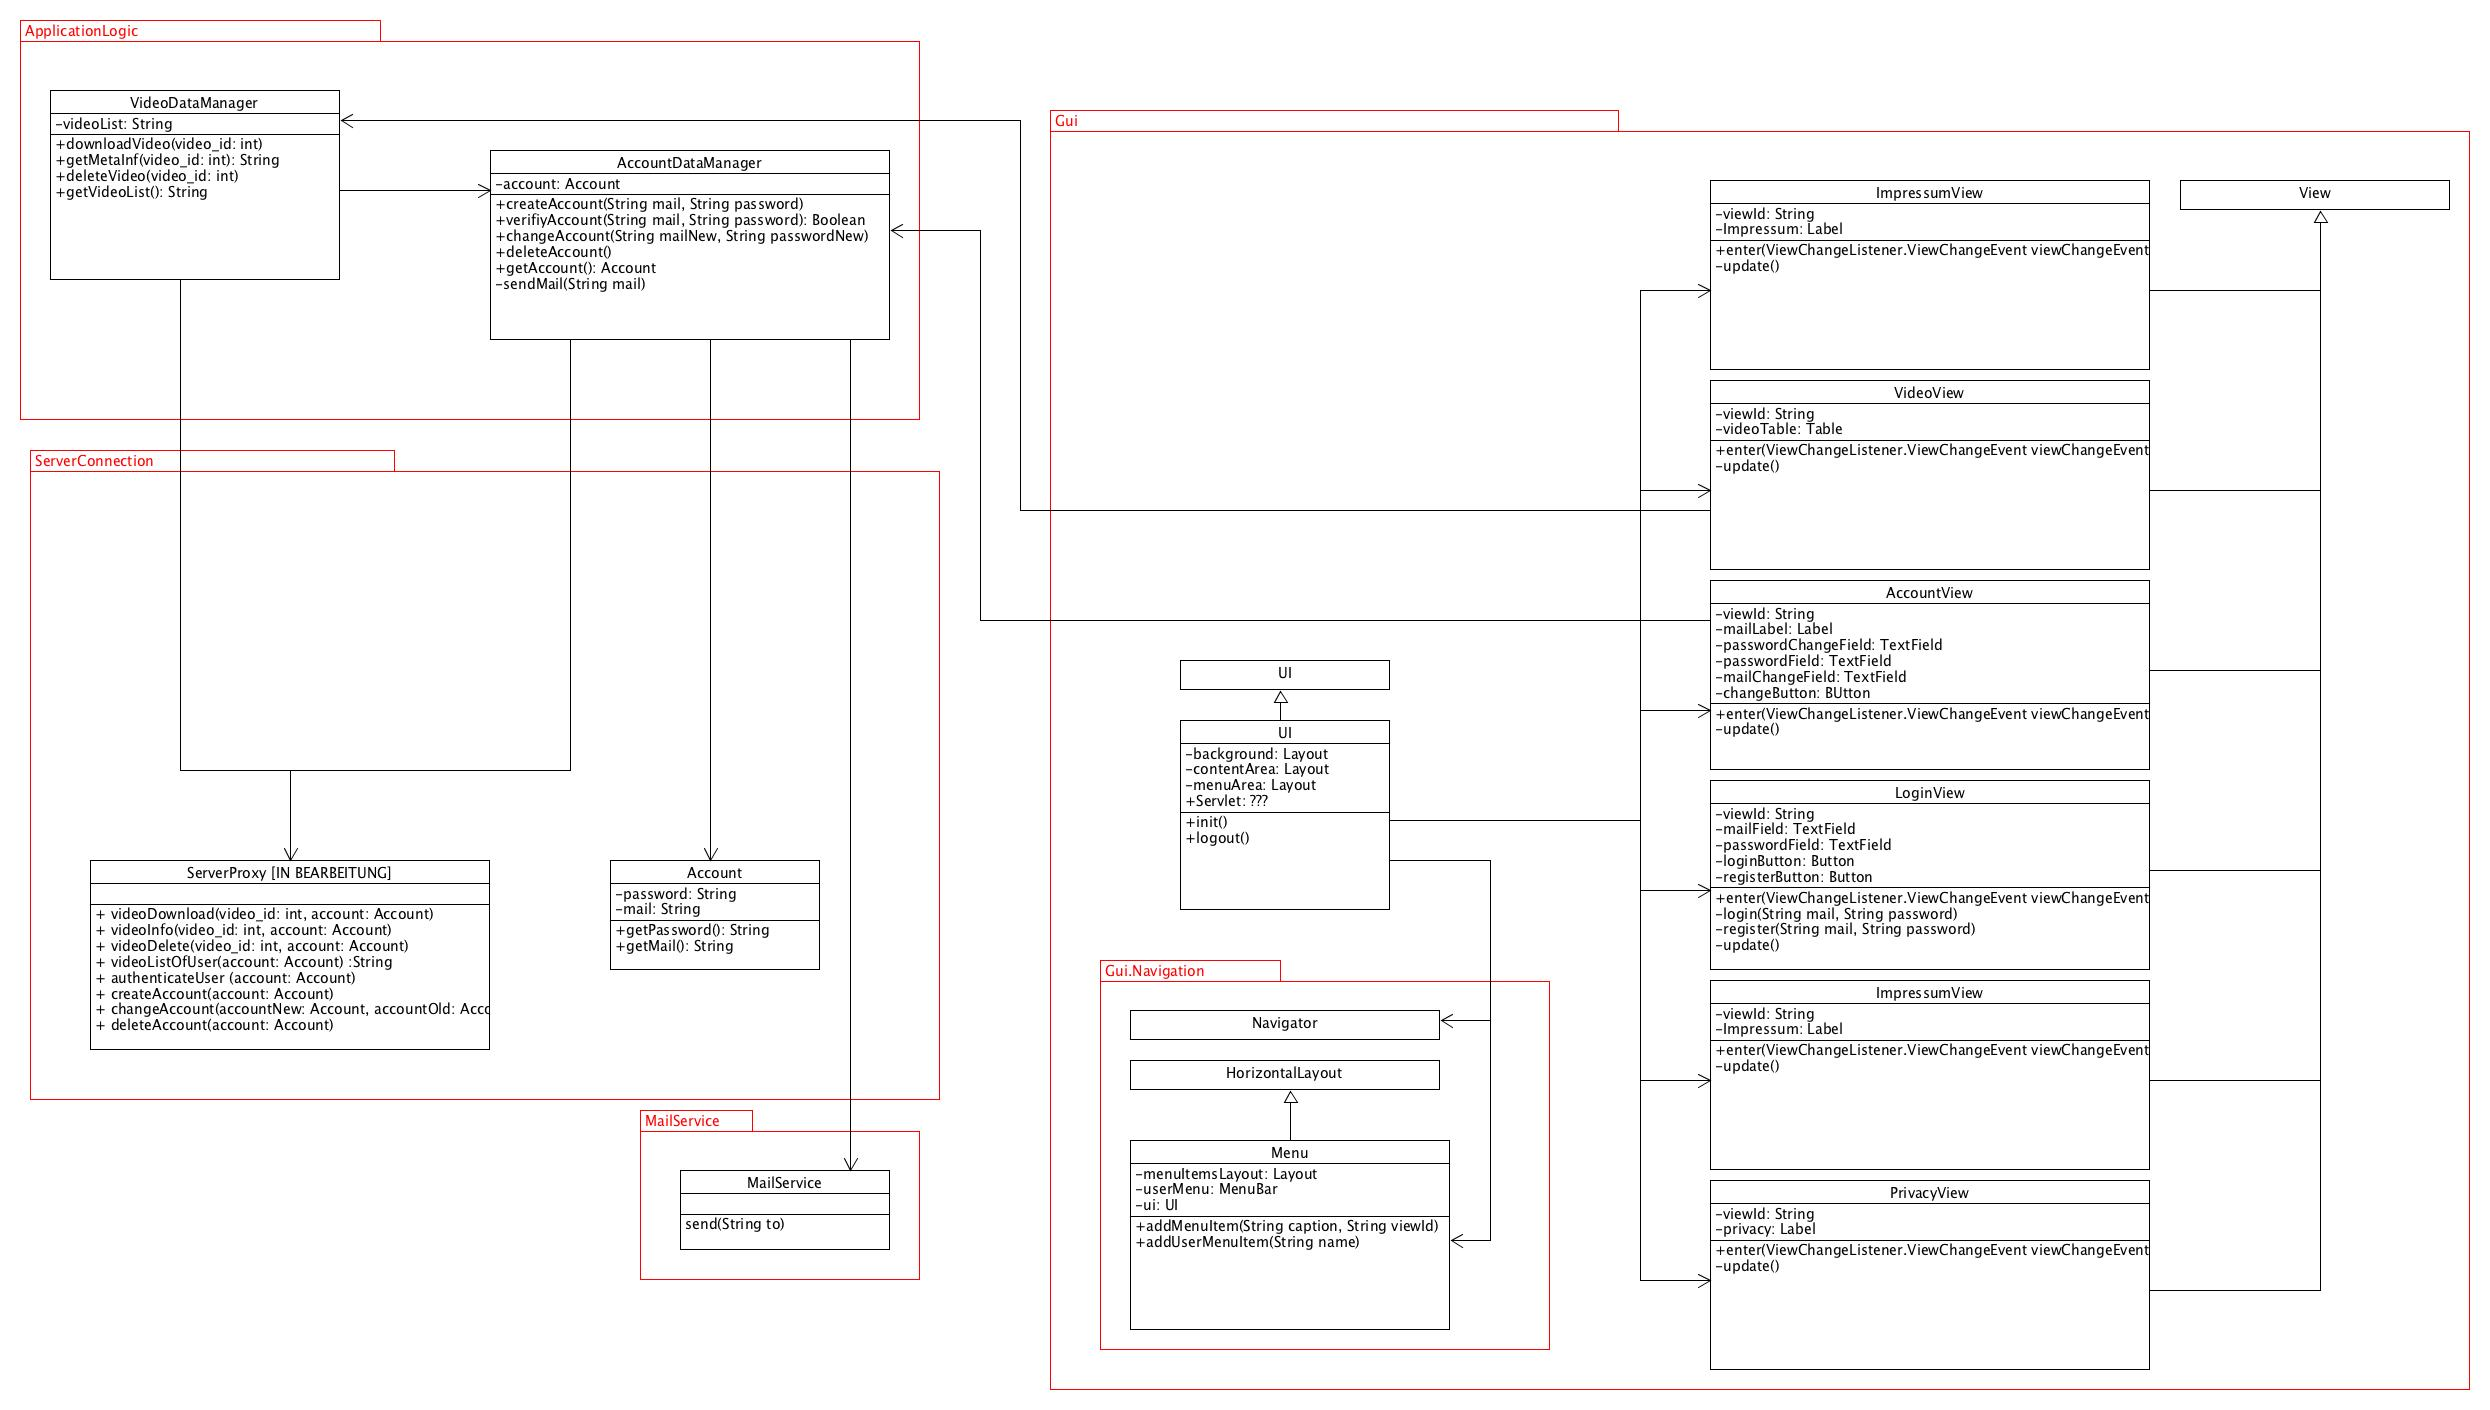
\includegraphics[width=1\textwidth]{./resources/Diagramme/WebInterface/UMLWebInterface.jpg}
\caption{UML Diagramm des Web-Interface}
	\label{interface:fig:modules_overview}
\end{figure}

\subsection{Entwurfsmuster}
Im Web-Interface wurden Entwurfsmuster verwendet um austauschbare Klassen zu erhalten. Zudem helfen sie dabei das Hinzufügen neuer Funktionalität möglichst einfach zu gestalten, was bei der Umsetzung von Wunschkriterien durchaus von Bedeutung sein wird.

\subsubsection{Proxy}
Da die Datenmanager Daten vom Web-Dienst holen müssen, wurde hier ein Proxy, der ServerProxy, zwischengeschalten um den Zugriff zu regeln. Des Weiteren werden so die Klassen des DataManagement Moduls vom Web-Dienst entkoppelt.

\subsubsection{Zustandsmuster}
Der Navigator verwendet ein Zustandsmuster um die Views anzuzeigen. Die verschiedenen Views entsprechen dabei den States.

\subsubsection{Schablonenmethode}
Die Klasse VideoDataManager verwendet eine Schablonenmethode zum erzeugen der Video Liste. In dieser werden die Videos und die Informationen vom Server geholt und dann entsprechend verarbeitet.
\newpage

\section{Modulübersicht} \label{interface:modul}
Die Komponente Web-Interface bietet dem Benutzer eine Schnittstelle zu unserem Web-Dienst, über die er Videos herunterladen und seinen Account verwalten kann. 

\subsection{Gui}
Die graphische Oberfläche besteht aus verschiedenen Views, wobei beim Start immer die LoginView angezeigt wird. 

\subsection{Gui.Navigation}
Die Navigation wird durch ein Menü und einen Navigator realisiert. Das Menü bietet dem Benutzer die Möglichkeit, die View zu wechseln. Den eigentlichen Wechsel übernimmt dann der Navigator.

\subsection{DataManagement}
Die beiden Manager (VideoDataManager, AccountDataManager siehe Klassenübersicht) bereiten Daten auf und kommunizieren über den ServerProxy mit dem Web-Dienst.

\subsection{ServerConnection}
Der ServerProxy übernimmt alle Zugriffe auf den Web-Dienst.

\subsection{MailService}
Eine Klasse, die die Aufgabe hat, die Verifizierungsmail zu senden.
\newpage


\section{Klassenübersicht}

\subsection{Gui}
\subsubsection{MyUI}\label{MyUI}
\textbf{extends} UI \newline
Die UI Klasse bildet das Herzstück des Webinterface. Die init Methode dieser Klasse wird beim Öffnen des Web-Interface aufgerufen. Diese Klasse hat die Aufgabe, alle Komponenten zu initialisieren und bildet dazu die Grundlage für alle graphischen Einheiten.
\newline

\underline{Attribute}
\begin{itemize}
\itemsep0pt

\item \textbf{background: VerticalLayout} \hfill\\ 
\textbf{Sichtbarkeit} private

Der Background ist die Grundlage der graphischen Oberfläche des Web-Interface. Auf dem Background werden entweder menuArea und contentArea gelegt, oder beim Login die \nameref{LoginView}. Dieses Attribut wird in der init() Methode erzeugt und initialisiert.

\item \textbf{menuArea: VerticalLayout} \hfill\\ 
\textbf{Sichtbarkeit} private

Die menuArea ist die Grundlage für das \nameref{Menu}. Dieses Attribut wird in der init() Methode erzeugt und initialisiert.

\item \textbf{contentArea: VerticalLayout} \hfill\\ 
\textbf{Sichtbarkeit} private

Die contentArea ist die Grundlage für die Ansichten. Dieses Attribut wird in der init() Methode erzeugt und initialisiert.

\item \textbf{menu: Menu} \hfill\\
\textbf{Sichtbarkeit} private
 
Das Menu bildet die Steuereinheit für den Benutzer. Der Navigator wird in der init() Methode erzeugt und initialisiert.

\item \textbf{navigator: Navigator} \hfill\\ 
\textbf{Sichtbarkeit} private

Der Navigator hat die Aufgabe, die verschiedenen Ansichten in die contentArea zu laden. Der Navigator wird in der init() Methode erzeugt und initialisiert.

\end{itemize}

\underline{Methoden}
\begin{itemize}
\itemsep0pt
\item \textbf{init (request: VaadinRequest): void}\hfill\\
\textbf{Sichtbarkeit} protected

In dieser Methode wird zuerst die Grundlage für die graphische Oberfläche erzeugt. Dann werden alle graphischen Komponenten, der Navigator und das Menu erzeugt und initialisiert. Am Schluss wird noch die LoginView angezeigt.

\item \textbf{logout (): void}\hfill\\
\textbf{Sichtbarkeit} public

Diese Methode löscht die Account Daten aus dem \nameref{AccountDataManager} und zeigt die LoginView an.

\end{itemize}

\newpage
\newpage
\subsubsection{LoginView}\label{LoginView}
\textbf{extends}  VerticalLayout \newline
\textbf{implements} View \newline
Diese Klasse erbt von einem Layout, da sie selbst als graphische Komponente verwendet wird. Die \nameref{LoginView} wird bei jedem Start des Web-Interface oder nach einem Logout angezeigt. Nach erfolgreichem Login leitet sie diese Information an eine übergeordnete Komponente weiter.
\newline

\underline{Attribute}
\begin{itemize}
\itemsep0pt
\item \textbf{viewId: String} \hfill\\ 
\textbf{Sichtbarkeit} private

Die viewId gibt der View eine einzigartige ID über die der Navigator die View identifizieren kann.

\item \textbf{mailField: TextField} \hfill\\ 
\textbf{Sichtbarkeit} private

Ein einfaches Eingabefeld zur Eingabe der Mail-Adresse.

\item \textbf{passwordField: TextField} \hfill\\
\textbf{Sichtbarkeit} private

Ein einfaches Eingabefeld zur Eingabe des Passwortes.

\item \textbf{loginButton: Button} \hfill\\
Dieser Button sendet Mail-Adresse und Passwort an den AccountDataManager zum verifizieren.

\item \textbf{registerButton: Button} \hfill\\
\textbf{Sichtbarkeit} private

Dieser Button sendet Mail-Adresse und Passwort an den \nameref{AccountDataManager} zum erzeugen eines neuen \nameref{Account}s.

\end{itemize}

\underline{Konstruktoren}
\begin{itemize}
\itemsep0pt
\item \textbf{LoginView(ui: \nameref{MyUI})} \hfill\\
\textbf{Sichtbarkeit} public

Durch die Referenz auf die UI wird nach erfolgreichem Login das \nameref{Menu} und die \nameref{VideoView} geladen.
\end{itemize}

\underline{Methoden}
\begin{itemize}
\itemsep0pt
\item \textbf{enter (viewChangeEvent: ViewChangeListener.ViewChangeEvent): void}\hfill\\
\textbf{Sichtbarkeit} public

Diese Methode wird immer bei Eintreten der View aufgerufen.

\item \textbf{update (): void}\hfill\\
\textbf{Sichtbarkeit} public

Diese Methode wird zum Aktualisieren der View verwendet.

\item \textbf{login (mail: String, password: String): Boolean} \hfill\\ 
\textbf{Sichtbarkeit} private

Diese Methode wird vom loginButton aufgerufen. Sie sendet zur Überprüfung Mail und Passwort and den AccountDataManager. Bei Erfolg wird true zurückgegeben.

\item \textbf{register (mail: String, password: String): Boolean}\hfill\\
\textbf{Sichtbarkeit} private

Diese Methode wird vom registerButton aufgerufen. Sie sendet Mail und Passwort and den AccountDataManager zur Erstellung eines Accounts. Bei Erfolg wird true zurückgegeben.

\end{itemize}

\newpage
\newpage
\subsubsection{VideoView}\label{VideoView}
\textbf{extends}  VerticalLayout \newline
\textbf{implements} View \newline
Diese Klasse erbt von einem Layout, da sie selbst als graphische Komponente verwendet wird. Diese View dient zum Anzeigen der \nameref{Video}s, die ein Benutzer mit seiner App hochgeladen hat. Zur Anzeige selbst lädt diese Klasse einen \nameref{VideoTable}.
\newline

\underline{Attribute}
\begin{itemize}
\itemsep0pt
\item \textbf{viewId: String} \hfill\\ 
\textbf{Sichtbarkeit} private

Die viewId gibt der View eine einzigartige ID, mit welcher der Navigator die View identifizieren kann.

\end{itemize}

\underline{Konstruktoren}
\begin{itemize}
\itemsep0pt
\item \textbf{VideoView()} \hfill\\
\textbf{Sichtbarkeit} public

Standardkonstruktor
\end{itemize}

\underline{Methoden}
\begin{itemize}
\itemsep0pt
\item \textbf{enter (viewChangeEvent: ViewChangeListener.ViewChangeEvent) :void}\hfill\\
\textbf{Sichtbarkeit} public

Diese Methode wird immer bei Eintreten der View aufgerufen.

\item \textbf{update () :void}\hfill\\
\textbf{Sichtbarkeit} public

Diese Methode wird zum Aktualisieren der View verwendet.

\end{itemize}

\newpage
\newpage
\subsubsection{AccountView}\label{AccountView}
\textbf{extends}  VerticalLayout \newline
\textbf{implements} View \newline
Diese Klasse erbt von einem Layout, da sie selbst als graphische Komponente verwendet wird. Diese View dient zur Anzeige der aktuellen Accountdaten und zum Durchführen von Änderungen an diesen.
\newline

\underline{Attribute}
\begin{itemize}
\itemsep0pt
\item \textbf{viewId: String} \hfill\\
\textbf{Sichtbarkeit} private
 
Die viewId gibt der View eine einzigartige ID, über die der Navigator die View identifizieren kann.

\item \textbf{mailLabel: Label} \hfill\\ 
\textbf{Sichtbarkeit} private

Dieses Label dient zur Anzeige der derzeit gültigen Mail-Adresse des aktuell eingeloggten \nameref{Account}s.

\item \textbf{passwordChangeField: TextField} \hfill\\ 
\textbf{Sichtbarkeit} private

In diesem Eingabefeld kann bei Wunsch zur Änderung des Passwortes ein neues Passwort eingegeben werden.

\item \textbf{passwordField: TextField} \hfill\\ 
\textbf{Sichtbarkeit} private

Für alle gewünschten Änderungen muss hier das aktuell aktive Passwort eingegeben werden.

\item \textbf{mailChangeField: TextField} \hfill\\ 
\textbf{Sichtbarkeit} private

In diesem Eingabefeld kann bei Wunsch zur Änderung der Mail-Adresse eine neue eingegeben werden

\item \textbf{changeButton: Button} \hfill\\
\textbf{Sichtbarkeit} private

Durch Drücken dieses Buttons werden die Änderungsdaten an den \nameref{AccountDataManager} zur Bearbeitung geschickt.
\end{itemize}

\underline{Konstruktoren}
\begin{itemize}
\itemsep0pt
\item \textbf{AccountView()} \hfill\\
\textbf{Sichtbarkeit} public

Standardkonstruktor
\end{itemize}

\underline{Methoden}
\begin{itemize}
\itemsep0pt
\item \textbf{enter (viewChangeEvent: ViewChangeListener.ViewChangeEvent): void}\hfill\\
\textbf{Sichtbarkeit} public

Diese Methode wird immer bei Eintreten der View aufgerufen.

\item \textbf{update (): void}\hfill\\
\textbf{Sichtbarkeit} public

Diese Methode wird zum Aktualisieren der View verwendet.

\end{itemize}

\newpage
\newpage
\subsubsection{ImpressumView}\label{ImpressumView}
\textbf{extends}  VerticalLayout \newline
\textbf{implements} View \newline
Diese Klasse erbt von einem Layout, da sie selbst als graphische Komponente verwendet wird. Diese View hat nur die Aufgabe, das Impressum anzuzeigen. \newline

\underline{Attribute}
\begin{itemize}
\itemsep0pt
\item \textbf{viewId: String} \hfill\\ 
\textbf{Sichtbarkeit} private

Die viewId gibt der View eine einzigartige ID über die der Navigator die View identifizieren kann.

\item \textbf{impressum: Label} \hfill\\ 
\textbf{Sichtbarkeit} private

Dieses Label wird verwendet um das Impressum anzuzeigen.

\end{itemize}

\underline{Konstruktoren}
\begin{itemize}
\itemsep0pt
\item \textbf{ImpressumView()} \hfill\\
\textbf{Sichtbarkeit} public

Standardkonstruktor
\end{itemize}

\underline{Methoden}
\begin{itemize}
\itemsep0pt
\item \textbf{enter (viewChangeEvent: ViewChangeListener.ViewChangeEvent): void}\hfill\\
\textbf{Sichtbarkeit} public

Diese Methode wird immer bei Eintreten der View aufgerufen.

\item \textbf{update (): void}\hfill\\
\textbf{Sichtbarkeit} public

Diese Methode wird zum Aktualisieren der View verwendet.

\end{itemize}

\newpage
\newpage
\subsubsection{PrivacyView}\label{PrivacyView}
\textbf{extends}  VerticalLayout \newline
\textbf{implements} View \newline
Diese Klasse erbt von einem Layout, da sie selbst als graphische Komponente verwendet wird. Diese View hat nur die Aufgabe, die Datenschutzinformationen anzuzeigen.
\newline

\underline{Attribute}
\begin{itemize}
\itemsep0pt
\item \textbf{viewId: String} \hfill\\ 
\textbf{Sichtbarkeit} private

Die viewId gibt der View eine einzigartige ID über die der Navigator die View identifizieren kann.

\item \textbf{privacy: Label} \hfill\\ 
\textbf{Sichtbarkeit} private

Dieses Label wird verwendet, um die Datenschutzinformationen anzuzeigen.

\end{itemize}

\underline{Konstruktoren}
\begin{itemize}
\itemsep0pt
\item \textbf{PrivacyView()} \hfill\\
\textbf{Sichtbarkeit} public

Standardkonstruktor
\end{itemize}

\underline{Methoden}
\begin{itemize}
\itemsep0pt
\item \textbf{enter (viewChangeEvent: ViewChangeListener.ViewChangeEvent): void}\hfill\\
\textbf{Sichtbarkeit} public

Diese Methode wird immer beim Eintreten der View aufgerufen.

\item \textbf{update (): void}\hfill\\
\textbf{Sichtbarkeit} public

Diese Methode wird zum Aktualisieren der View verwendet.

\end{itemize}

\newpage
\subsubsection{VideoTable}\label{VideoTable}
\textbf{extends}  Table \newline
Jede Zeile des VideoTables beinhaltet ein \nameref{Video} mit den zugehörigen Buttons zum Downloaden, Löschen und Anzeigen der Infos. \newline

\underline{Attribute}
\begin{itemize}
\itemsep0pt

\item \textbf{downloadButtonList: LinkedList} \hfill\\ 
\textbf{Sichtbarkeit} private

Eine Liste an Buttons. Zu jedem Video wird ein Button erzeugt und an die Liste gehängt.

\item \textbf{infoButtonList: LinkedList} \hfill\\ 
\textbf{Sichtbarkeit} private

Eine Liste an Buttons. Zu jedem Video wird ein Button erzeugt und an die Liste gehängt.

\item \textbf{deleteButtonList: LinkedList} \hfill\\ 
\textbf{Sichtbarkeit} private

Eine Liste an Buttons. Zu jedem Video wird ein Button erzeugt und an die Liste gehängt.

\item \textbf{videos: LinkedList} \hfill\\
\textbf{Sichtbarkeit} private
 
Das Attribut ist eine Liste der Videos. Die Videos werden bei Erzeugen oder Updaten des Tables vom \nameref{VideoDataManager} geholt und dann verarbeitet.
\end{itemize}

\underline{Konstruktoren}
\begin{itemize}
\itemsep0pt

\item \textbf{VideoTable()} \hfill\\ 
\textbf{Sichtbarkeit} public

Im Konstruktor werden die Videos über den VideoDataManager geholt. Zudem werden dann für jedes Video die Buttons vorbereitet.

\end{itemize}


\underline{Methoden}
\begin{itemize}
\itemsep0pt

\item \textbf{prepareVideos (): void}\hfill\\
\textbf{Sichtbarkeit} private

Die Videos werden zur Anzeige vorbereitet.

\item \textbf{prepareButtons (): void}\hfill\\
\textbf{Sichtbarkeit} private

Die Buttons werden zur Anzeige vorbereitet, d.h. es werden Name und Listener gesetzt.

\item \textbf{update (): void}\hfill\\
\textbf{Sichtbarkeit} public

Dies Methode wird verwendet um den Table zu aktualisieren.

\end{itemize}

\newpage
\subsection{Gui.Navigation}
\subsubsection{Menu}\label{Menu}
\textbf{extends}  HorizontalLayout \newline
Das Menu stellt die Buttons bereit, die benötigt werden, um den Benutzer zwischen den verschiedenen Ansichten wechseln zu lassen. Dazu kommt noch der Logout Button, über den man zurück zum Login gelangt.
\newline

\underline{Attribute}
\begin{itemize}
\itemsep0pt

\item \textbf{menuItemLayout: Layout} \hfill\\ 
\textbf{Sichtbarkeit} private

In dieses Layout werden neu erstellte Menu-Items hinzugefügt.

\item \textbf{userMenu: MenuBar} \hfill\\ 
\textbf{Sichtbarkeit} private

Eine Referenz auf das userMenu.

\item \textbf{ui: \nameref{MyUI}} \hfill\\ 
\textbf{Sichtbarkeit} private

Eine Referenz auf die ui in der das Menu liegt. Dies wird verwendet um den Navigator aufzurufen und den Logout durchzuführen.

\end{itemize}

\underline{Konstruktoren}
\begin{itemize}
\itemsep0pt
\item \textbf{Menu()} \hfill\\
\textbf{Sichtbarkeit} public

Standardkonstruktor
\end{itemize}

\underline{Methoden}
\begin{itemize}
\itemsep0pt
\item \textbf{addMenuItem (caption: String, viewId: String): void}\hfill\\
\textbf{Sichtbarkeit} public

Diese Methode dient zum Einfügen neuer Menüeinträge, die einen Ansichtswechsel auslösen sollen.

\item \textbf{addUserMenu (name: String): void}\hfill\\
\textbf{Sichtbarkeit} public

Diese Methode dient zum Einfügen eines User-Menüs. Es kann immer nur ein User-Menü geben.

\item \textbf{addLogoutItem (): void}\hfill\\
\textbf{Sichtbarkeit} public

Diese Methode dient zum Einfügen eines Logout-Eintrages. Dieser Eintrag ruft dann den Logout der übergeordneten \nameref{MyUI} auf.

\end{itemize}

\newpage
\subsection{DataManagement}
\subsubsection{AccountDataManager}\label{AccountDataManager}
Die Klasse dient zur Accountdatenverwaltung und Kommunikation mit dem \nameref{ServerProxy}. Dazu bereitet sie Daten in beide Richtungen auf. \newline

\underline{Attribute}
\begin{itemize}
\itemsep0pt

\item \textbf{account: \nameref{Account}} \hfill\\ 
\textbf{Sichtbarkeit} private \newline
\textbf{statisch}

Eine Referenz auf den Account, der in dieser Sitzung eingeloggt wurde.

\end{itemize}

\underline{Methoden}
\begin{itemize}
\itemsep0pt
\item \textbf{createAccount (mail: String, password: String): String}\hfill\\
\textbf{Sichtbarkeit} public \newline
\textbf{Statisch}

Eine Methode, die Eingaben der \nameref{LoginView} bekommt und diese dann an den ServerProxy in der jeweiligen Methode weitergibt.

\item \textbf{startVerification (mail: String, password: String): void}\hfill\\
\textbf{Sichtbarkeit} private \newline
\textbf{Statisch}

Diese Methode wird nach dem Registrieren aufgerufen. Sie erzeugt eine UUID und sendet diese einmal in einem Link per Mail an den Benutzer und dann noch an den ServerProxy.

\item \textbf{authenticteAccount (account: Account): boolean}\hfill\\
\textbf{Sichtbarkeit} public \newline
\textbf{Statisch}

Diese Methode wird beim Login benutzt. Sie gibt an ob Passwort und Mail-Adresse korrekt sind.

\item \textbf{checkVerification (account: Account): boolean}\hfill\\
\textbf{Sichtbarkeit} public \newline
\textbf{Statisch}

Diese Methode wird beim Login benutzt. Sie gibt an ob ein Account verifiziert ist.

\item \textbf{changeAccount (mail: String, password: String): void}\hfill\\
\textbf{Sichtbarkeit} public \newline
\textbf{Statisch}

Eine Methode die Eingaben von der \nameref{AccountView} bekommt. Anschließend wird das Passwort mit dem derzeitigen Passwort verglichen. Bei Erfolg werden die Änderungen an den ServerProxy übergeben.

\item \textbf{deleteAccount (): void}\hfill\\
\textbf{Sichtbarkeit} public \newline
\textbf{Statisch}

Bei deleteAccount werden die derzeitigen Account-Daten an den ServerProxy in einem delete-Befehl übergeben. Anschließend werden die lokalen Account Daten gelöscht und die Seite neu geladen.

\item \textbf{sendMail (mail: String): void}\hfill\\
\textbf{Sichtbarkeit} private \newline
\textbf{Statisch}

Diese Funktion wird benutzt um Nutzern eine Mail zur Bestätigung nach Erstellen und Löschen eines Accounts zu senden.
\end{itemize}

\newpage
\newpage
\subsubsection{Account}\label{Account}
In dieser Klasse werden die Mail-Adresse und das Passwort eines Benutzers zu einem Account zusammengefasst. \newline

\underline{Attribute}
\begin{itemize}
\itemsep0pt
\item \textbf{mail: String} \hfill\\
\textbf{Sichtbarkeit} private
 
Ein String zum Speichern der Mail-Adresse.

\item \textbf{password: String} \hfill\\ 
\textbf{Sichtbarkeit} private

Ein String zum Speichern des Passwortes.

\end{itemize}

\underline{Konstruktoren}
\begin{itemize}
\itemsep0pt
\item \textbf{Account(String: mail, String: password)} \hfill\\
\textbf{Sichtbarkeit} public

Nimmt die Parameter und setzt die Attribute.
\end{itemize}

\newpage
\newpage
\subsubsection{VideoDataManager}\label{VideoDataManager}
Der VideoDataManager verwaltet die Videodaten und vereinfacht den Zugriff auf den \nameref{ServerProxy} für Klassen, die Videodaten benötigen. \newline

\underline{Attribute}
\begin{itemize}
\itemsep0pt

\item \textbf{videos: LinkedList}\hfill\\
\textbf{Sichtbarkeit} private \newline
\textbf{statisch}

Eine Liste in dem der VideoDataManager die \nameref{Video}s hält die er vom ServerProxy bekommt.
\end{itemize}

\underline{Methoden}
\begin{itemize}
\itemsep0pt


\item \textbf{downloadVideo (videoId: int): void}\hfill\\
\textbf{Sichtbarkeit} public \newline
\textbf{Statisch}

Die Methode fügt die \nameref{Account}-Daten hinzu und ruft danach die Methode zum downloaden am ServerProxy auf.

\item \textbf{deleteVideo (videoId: int): void}\hfill\\
\textbf{Sichtbarkeit} public \newline
\textbf{Statisch}

Die Methode fügt die Account-Daten hinzu und ruft am ServerProxy die Methode zum Löschen eines Videos auf.

\item \textbf{updateVideosAndInfo (): String}\hfill\\
\textbf{Sichtbarkeit} public \newline
\textbf{Statisch}

Die Methode fügt die Account Daten hinzu und ruft am ServerProxy die Methode auf, welcher die Videos zurückgibt. Anschließend wird parseVideos aufgerufen und die Videos als Attribut gespeichert.

\item \textbf{getVideosFromServer (): String}\hfill\\
\textbf{Sichtbarkeit} private \newline
\textbf{Statisch}

Die Methode schickt eine Anfrage an den ServerProxy zum Holen der Videos.

\item \textbf{createVideoList (videos: String): LinkedList}\hfill\\
\textbf{Sichtbarkeit} private \newline
\textbf{Statisch}

Diese Methode parst die Videos in Name und Id. Anschließend erstellt sie eine Liste aus Video Objekten.

\item \textbf{addInfoToVideoList (videos: LinkedList): LinkedList}\hfill\\
\textbf{Sichtbarkeit} private \newline
\textbf{Statisch}

Diese Methode fügt jedem Listeneintrag die Meta-Informationen hinzu.

\item \textbf{getMetaInfFromServer (videoId: int): String}\hfill\\
\textbf{Sichtbarkeit} private \newline
\textbf{Statisch}

Die Methode fügt die Account Daten hinzu und ruft am ServerProxy die Methode auf, die die Metadaten als String zurückgibt.

\end{itemize}
\newpage
\newpage
\subsubsection{Video}\label{Video}
In dieser Klasse werden Name, Id und die Meta-Informationen zu einem Video zusammgefasst. \newline

\underline{Attribute}
\begin{itemize}
\itemsep0pt
\item \textbf{name: String} \hfill\\
\textbf{Sichtbarkeit} private

Ein String zum Speichern des Namens.

\item \textbf{id: int} \hfill\\ 
\textbf{Sichtbarkeit} private

Ein Integer zum Speichern der Id.

\item \textbf{info: String} \hfill\\ 
\textbf{Sichtbarkeit} private

Ein String zum Speichern der Meta-Informationen.

\end{itemize}

\underline{Konstruktoren}
\begin{itemize}
\itemsep0pt
\item \textbf{Account(String: name, int: id, String: info)} \hfill\\
\textbf{Sichtbarkeit} public

Nimmt die Parameter und setzt damit die Attribute.
\end{itemize}

\newpage
\subsection{ServerConnection}
\subsubsection{ServerProxy}\label{ServerProxy}

Diese Klasse dient zur Kommunikation mit dem Web-Dienst. Sie ist die einzige Klasse, die mit dem Web-Dienst kommunizieren kann. \newline

\underline{Methoden}
\begin{itemize}
\itemsep0pt

\item \textbf{videoDownload (videoId: int, account: \nameref{Account}): Response}\hfill\\
\textbf{Sichtbarkeit} public \newline
\textbf{Statisch}

Die Methode sendet die Anfrage zum Download eines Videos an den Web-Dienst.

\item \textbf{videoInfo (videoId: int, account: Account): String}\hfill\\
\textbf{Sichtbarkeit} public \newline
\textbf{Statisch}

Die Methode holt die Metadaten eines Videos vom Web-Dienst.

\item \textbf{videoDelete (videoId: int, account: Account): String}\hfill\\
\textbf{Sichtbarkeit} public \newline
\textbf{Statisch}

Die Methode sendet die Anfrage zum Löschen eines Videos an den Web-Dienst.

\item \textbf{getVideosByAccount (account: Account): String}\hfill\\
\textbf{Sichtbarkeit} public \newline
\textbf{Statisch}

Die Methode sendet eine Anfrage an den Web-Dienst, um alle Videos des Accounts zu bekommen.

\item \textbf{authenticteUser (account: Account): String}\hfill\\
\textbf{Sichtbarkeit} public \newline
\textbf{Statisch}

Die Methode sendet eine Anfrage zum Überprüfen der Mitgegebenen Accountdaten. Zudem wird überprüft ob der Account verifiziert ist.

\item \textbf{setVerificationID (account: Account, verificationID: int): String}\hfill\\
\textbf{Sichtbarkeit} public \newline
\textbf{Statisch}

Die Methode sendet die zuvor erzeugte ID an den Web-Dienst, dass dieser sie mit der aus dem Link abgleichen kann.

\item \textbf{checkVerification (account: Account): String}\hfill\\
\textbf{Sichtbarkeit} public \newline
\textbf{Statisch}

Die Methode sendet die zuvor erzeugte ID an den Web-Dienst, dass dieser sie mit der aus dem Link abgleichen kann.

\item \textbf{createAccount (account: Account): String}\hfill\\
\textbf{Sichtbarkeit} public \newline
\textbf{Statisch}

Die Methode sendet die Anfrage zum Erzeugen eines Accounts an den Web-Dienst.

\item \textbf{changeAccount (accountNew: Account, accountOld: Account): String}\hfill\\
\textbf{Sichtbarkeit} public \newline
\textbf{Statisch}

Die Methode sendet die Anfrage zum Ändern eines Accounts an den Web-Dienst.

\item \textbf{deleteAccount (account: Account): String}\hfill\\
\textbf{Sichtbarkeit} public \newline
\textbf{Statisch}

Die Methode sendet die Anfrage zum Löschen eines Accounts an den Web-Dienst.

\end{itemize}

\newpage
\subsection{MailService}
\subsubsection{MailService}\label{MailService}
Diese Klasse dient zum Senden der Verifikationsmail. \newline


\underline{Methoden}
\begin{itemize}
\itemsep0pt
\item \textbf{send (String: to, String: content): void}\hfill\\
\textbf{Sichtbarkeit} public \newline
\textbf{Statisch}

Die Methode konfiguriert den SMTP und erzeugt eine Mail. Anschließend wird die Mail dann über den SMTP gesendet.

\end{itemize}




%PUT ATTACHMENTS HERE
\chapter{Anhang}

\section{Sequenzdiagramme}

\begin{figure}[ht]
	\centering
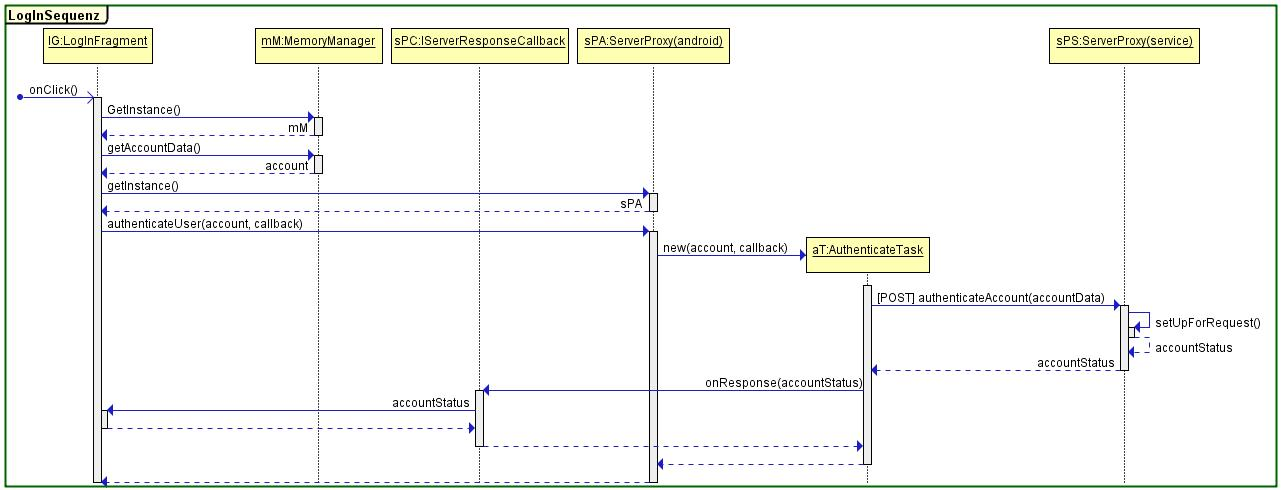
\includegraphics[width=1\textwidth]{./resources/Diagramme/App/logInSequence.jpg}
\caption{Anmelden in der App}
	\label{fig:AppAuth}
\end{figure}

\begin{figure}[ht]
	\centering
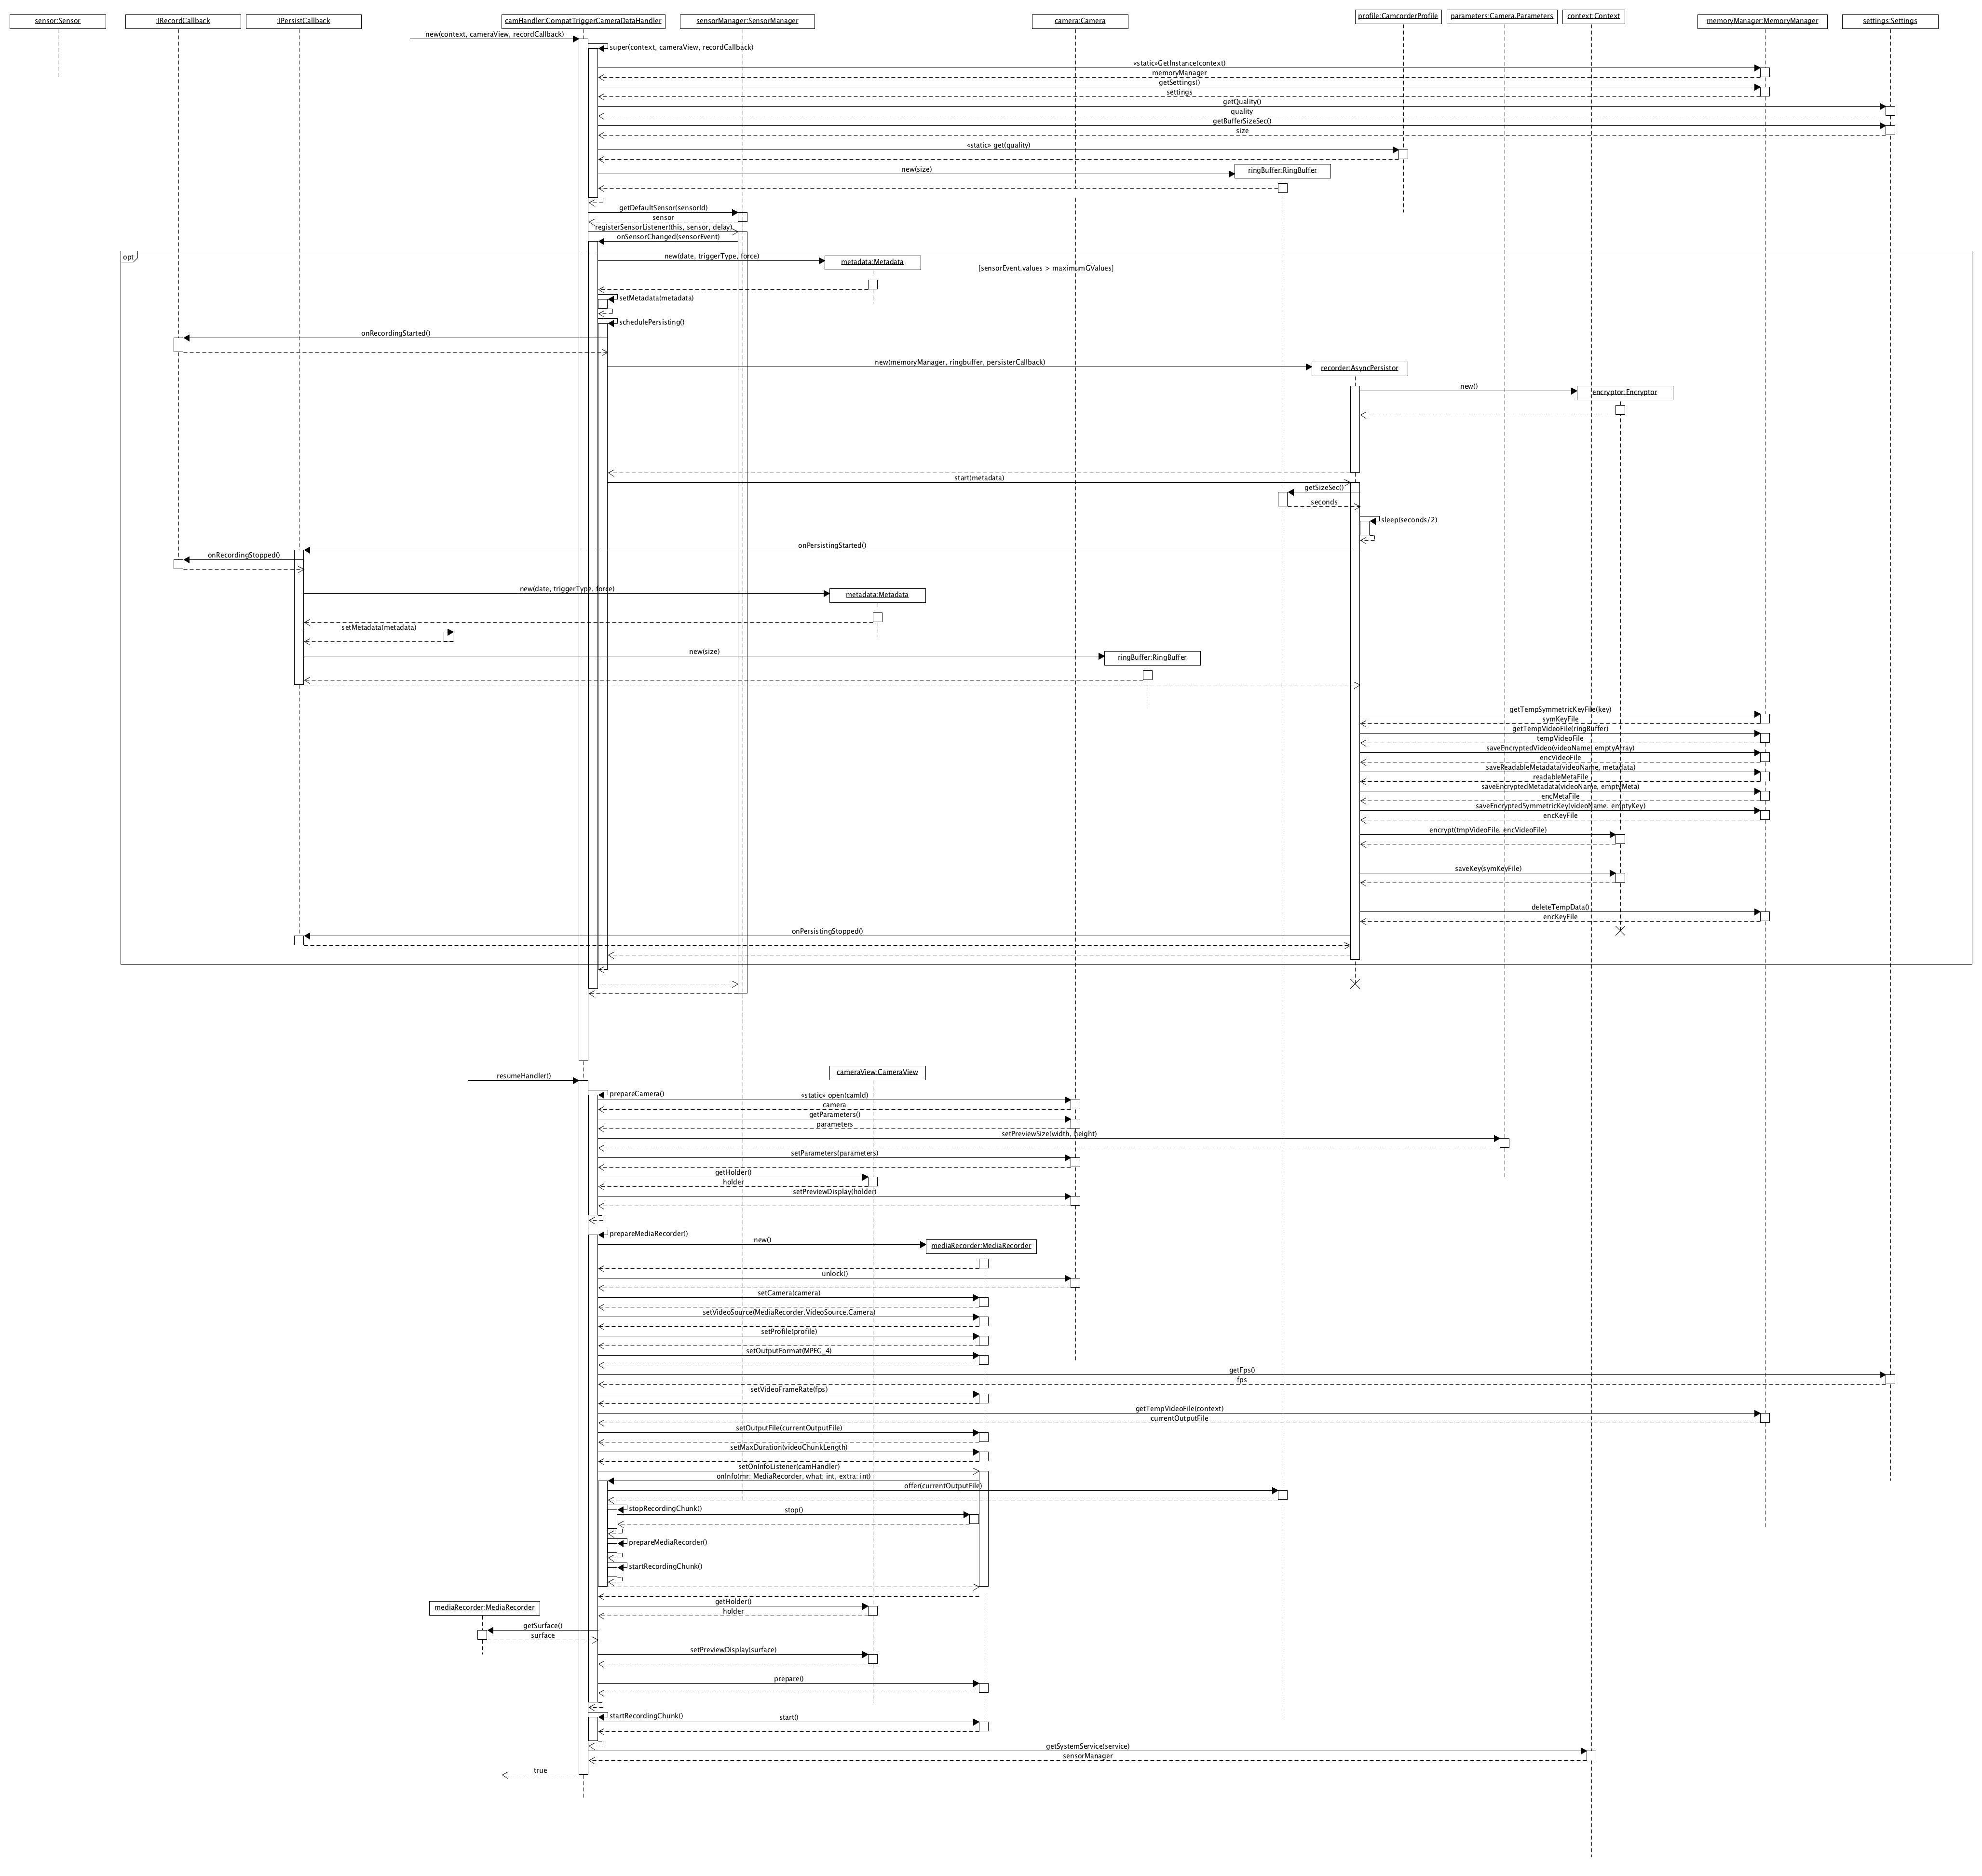
\includegraphics[width=1\textwidth]{./resources/Diagramme/App/recordSequence.jpg}
\caption{Videoaufnahme in der App}
	\label{fig:AppVideo}
\end{figure}

\begin{figure}[ht]
	\centering
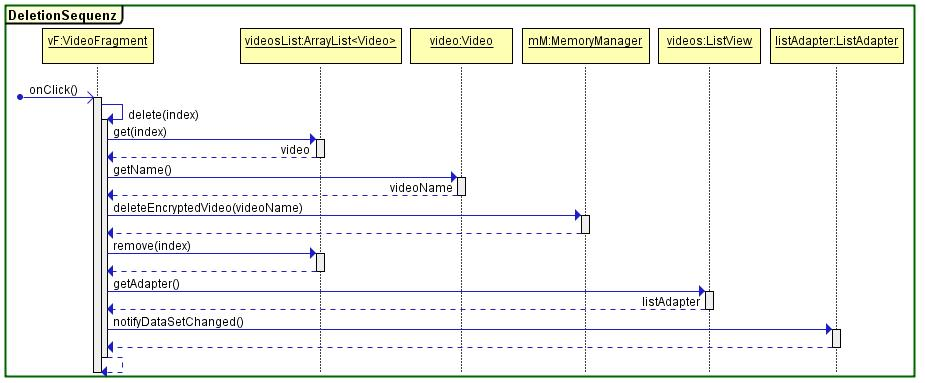
\includegraphics[width=1\textwidth]{./resources/Diagramme/App/deleteVideoSequence.jpg}
\caption{Video in der App löschen}
	\label{fig:AppDel}
\end{figure}

\begin{figure}[ht]
	\centering
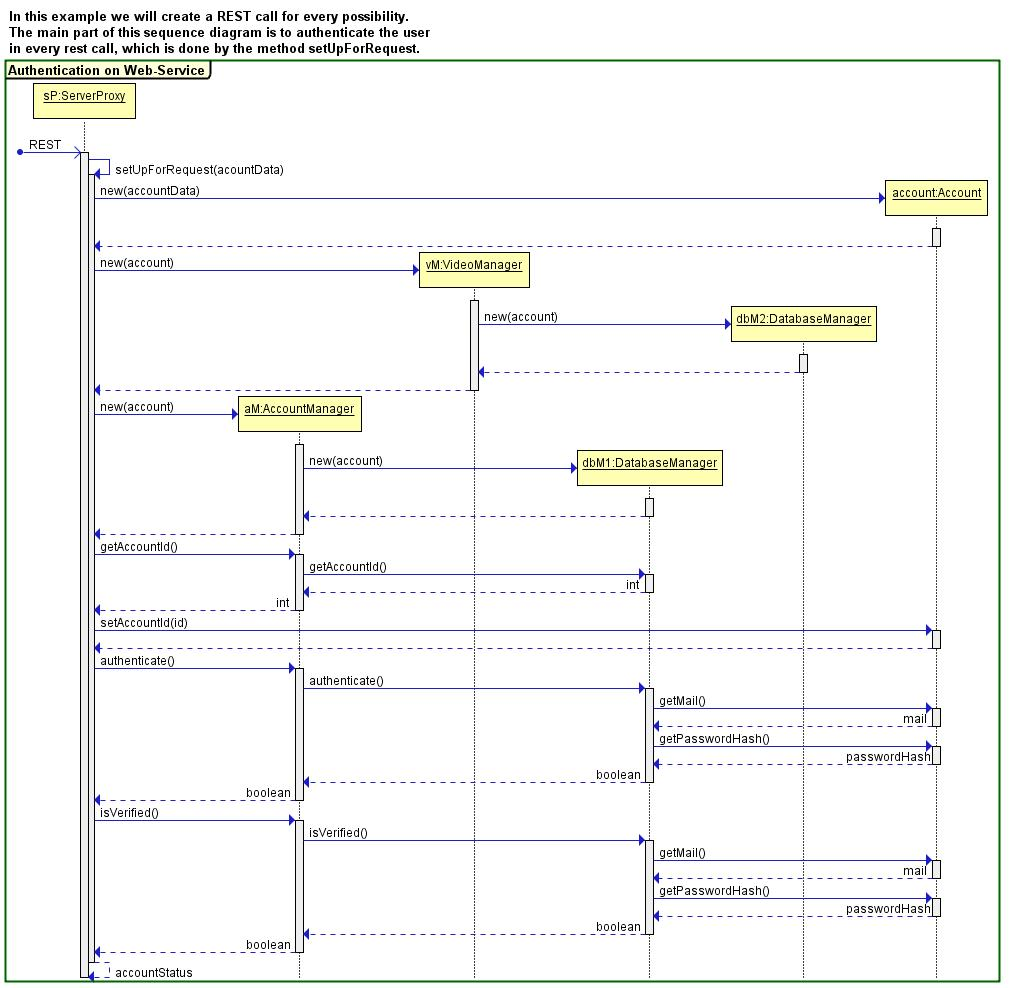
\includegraphics[width=1\textwidth]{./resources/Diagramme/Webservice/SeqAuthenticate.jpg}
\caption{Authentifizieren auf dem Dienst}
	\label{fig:ServiceAuth}
\end{figure}

\begin{figure}[ht]
	\centering
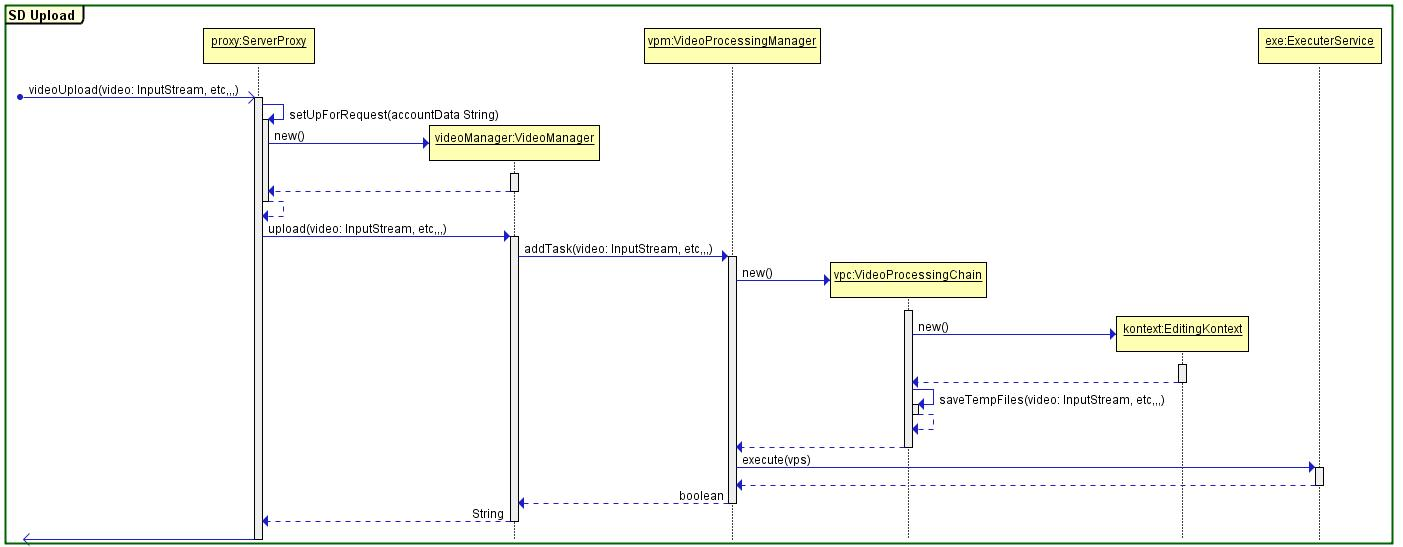
\includegraphics[width=1\textwidth]{./resources/Diagramme/Webservice/Upload.jpg}
\caption{Video auf den Dienst hochladen}
	\label{fig:ServiceUpload}
\end{figure}

\begin{figure}[ht]
	\centering
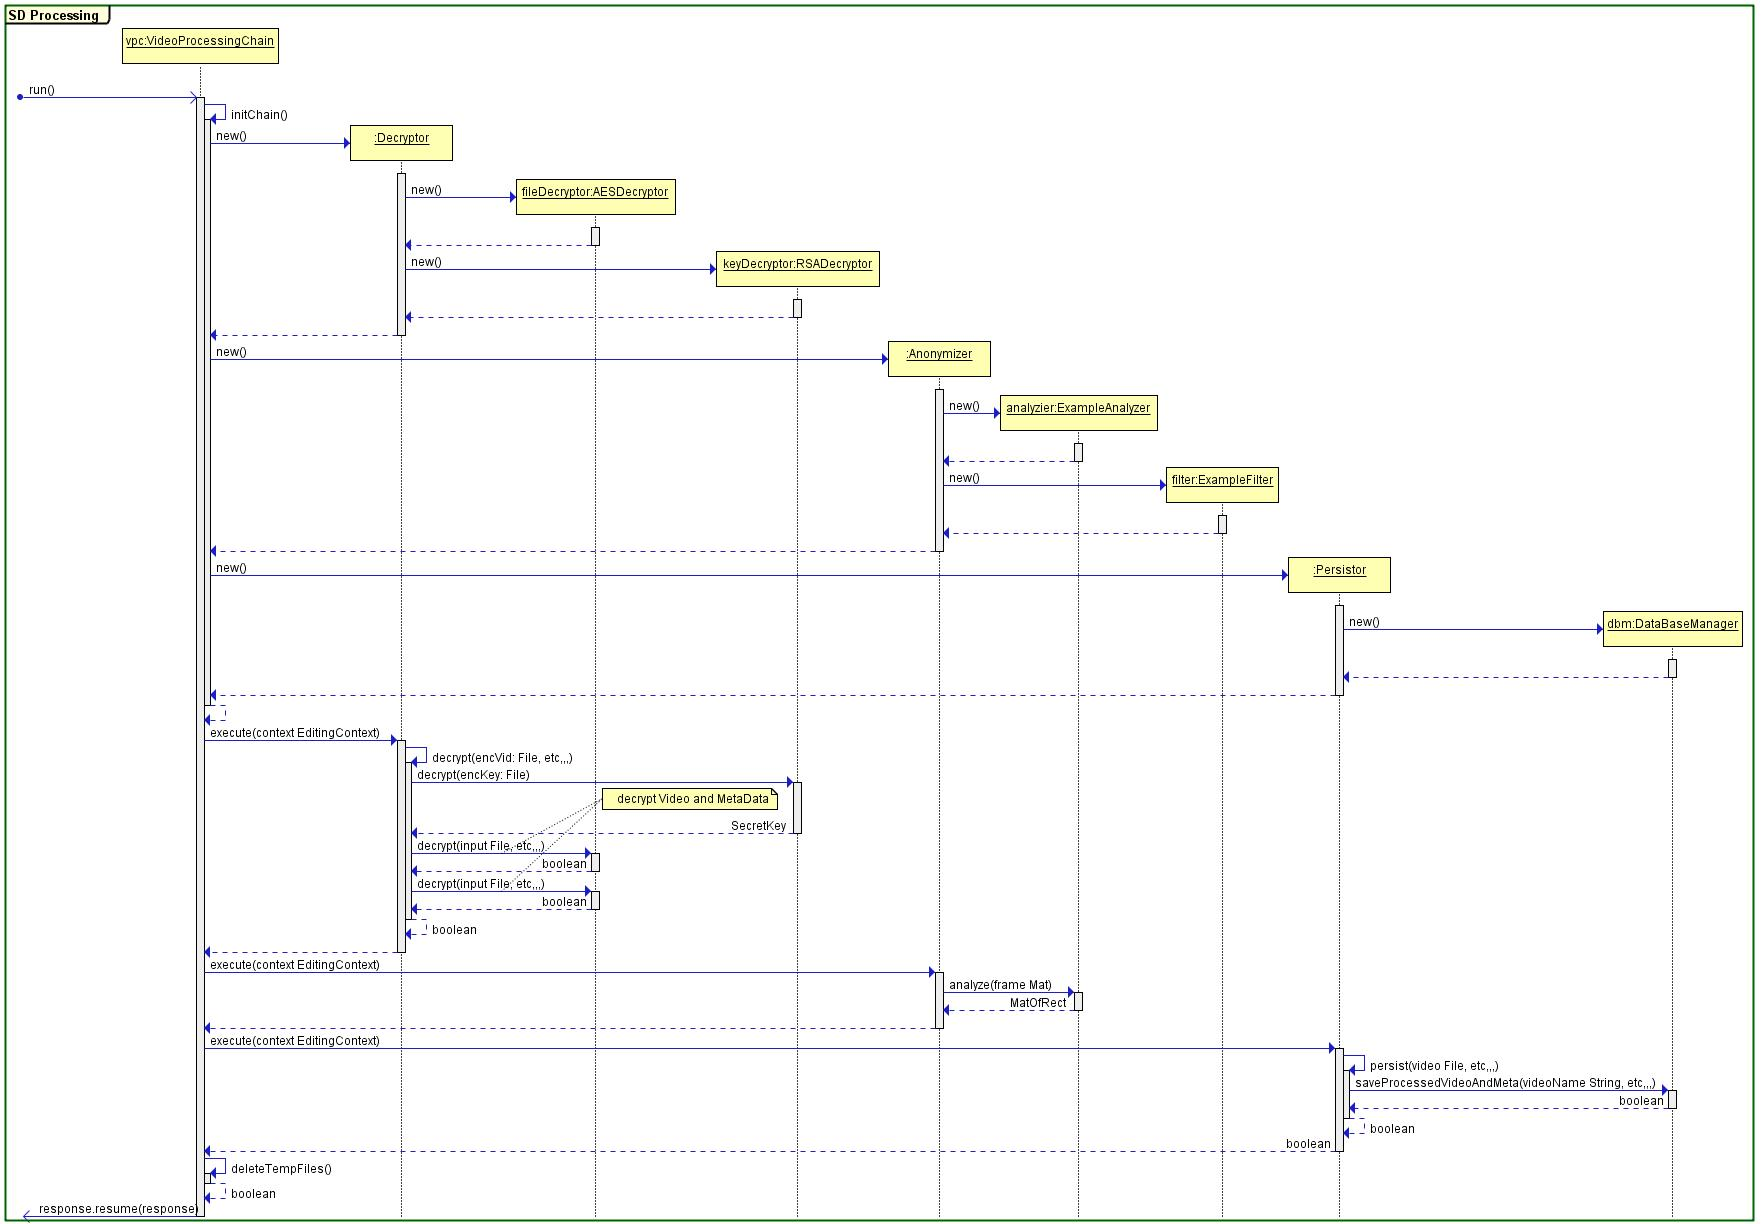
\includegraphics[width=1\textwidth]{./resources/Diagramme/Webservice/Processing.jpg}
\caption{Videobearbeitung auf dem Dienst}
	\label{fig:ServiceProcess}
\end{figure}

\begin{figure}[ht]
	\centering
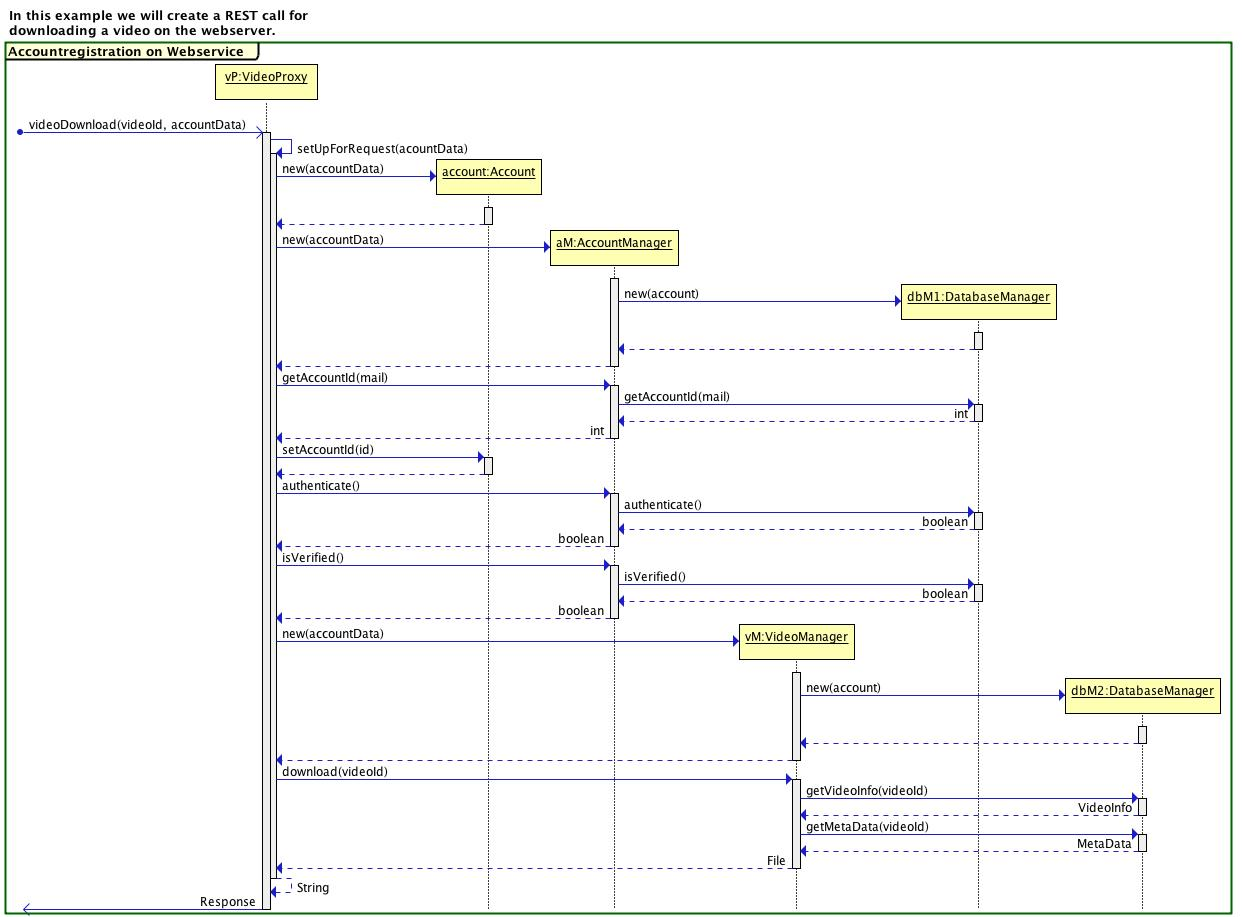
\includegraphics[width=1\textwidth]{./resources/Diagramme/Webservice/SeqVideoDownload.jpg}
\caption{Videodownload vom Dienst}
	\label{fig:ServiceDownl}
\end{figure}

\begin{figure}[ht]
	\centering
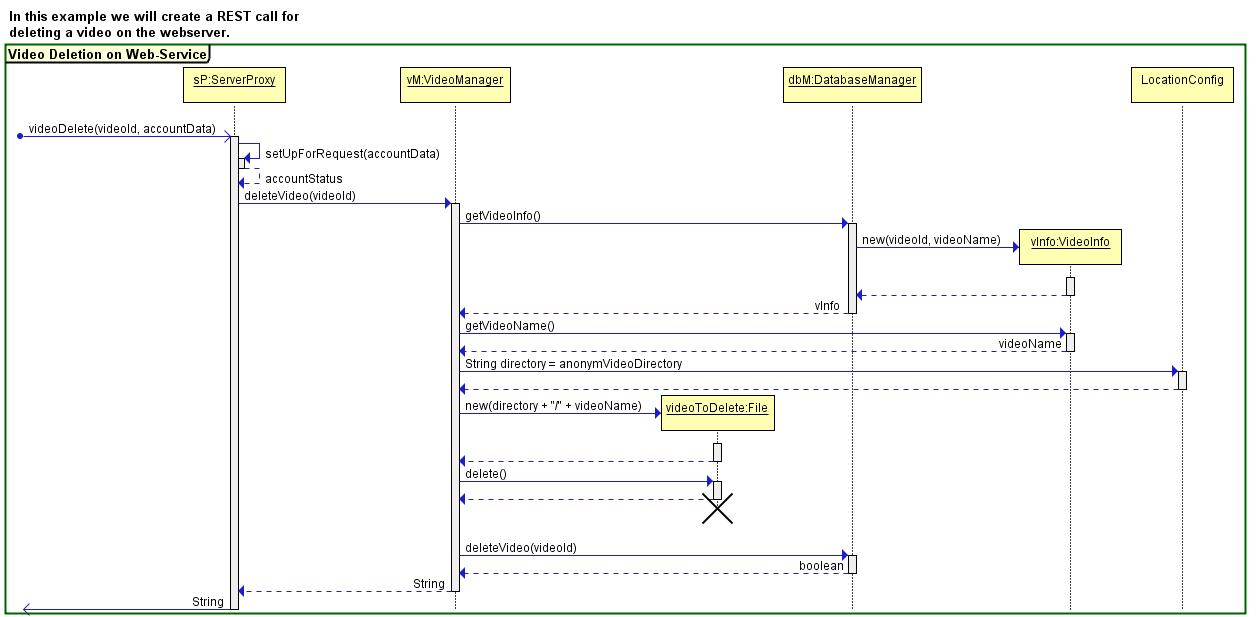
\includegraphics[width=1\textwidth]{./resources/Diagramme/Webservice/SeqVideoDeletion.jpg}
\caption{Video auf dem Dienst löschen}
	\label{fig:ServiceDel}
\end{figure}

%end content

\end{document}

